\documentclass[a4paper, 12pt]{report}
 
% Préambule du document
\usepackage[utf8]{inputenc}
\usepackage[T1]{fontenc}
%\usepackage[francais]{babel}
\usepackage[top=2cm, bottom=2cm, right=2.5cm, left=2.5cm]{geometry}

% Figures et légendes
\usepackage{graphicx}
\usepackage{wrapfig}
\usepackage{caption}
\usepackage{float}
\floatplacement{figure}{!h}

% Police
\usepackage{fontspec}
\setmainfont{Times New Roman}

% Tableaux
\usepackage{array}
\newcommand{\comment}[1]{}
\newcommand*{\thead}[1]{%
	% Entête des tableaux
	\centering\bfseries\arraybackslash #1
}

% Page de garde
%\usepackage{fullpage}
\title{Mémoire d'ingénieur}

% Titres des parties 
\usepackage[frenchb]{babel}
\addto\captionsfrench{\renewcommand{\chaptername}{Partie}}
\renewcommand{\thechapter}{\Roman{chapter}}
\renewcommand{\thesection}{\Alph{section})}
\renewcommand{\thesubsection}{\arabic{subsection})}

% Espacements
\renewcommand{\baselinestretch}{1.15}
\setlength{\parskip}{0.1cm}
\usepackage{titlesec}
%\titlespacing\chapter{0pt}{*-300pt}{0pt}

% Maths
\usepackage{amsmath}
\usepackage{amssymb}

% Ajoute un niveau de détail de titre à la table des matières
\setcounter{tocdepth}{3}
\setcounter{secnumdepth}{3}

% Annexes
\usepackage{appendix}
\newcommand{\nocontentsline}[3]{}
\newcommand{\tocless}[2]{\bgroup\let\addcontentsline=\nocontentsline#1{#2}\egroup}

% Gestion des différentes parties du document
\makeatletter
	\newcommand\frontmatter{%
	  \cleardoublepage
	  \thispagestyle{empty}
	}
	\newcommand\mainmatter{%
	  \cleardoublepage
	  \pagenumbering{arabic}
	}
	\newcommand\backmatter{%
	  \pagenumbering{roman}
	  \if@openright
	    \cleardoublepage
	  \else
	    \clearpage
	  \fi
	}
\makeatother

% biblio
\usepackage[round,authoryear]{natbib}
\usepackage{url}

\begin{document}
	\bibliographystyle{abbrvnat}
	%Amélioration d'une console de supervision d'un
EAI hospitalier : étude du besoin et implémentation technique

Medical context EAI oversight console improving : needs study and technical
implementation
	\begin{titlepage}
	\vfill
	\begin{figure}[H]
		\centering
		
\includegraphics[width=17cm]{../img/pageDeGarde.png}
	\end{figure}
	\vfill
	\end{titlepage}
	
	\newpage
	
	\frontmatter
	
	\thispagestyle{empty}
	\tableofcontents\thispagestyle{empty}
	\newpage
	
	\thispagestyle{empty}
	\listoffigures\thispagestyle{empty}
	\newpage	
	
	\thispagestyle{empty}
	\listoftables\thispagestyle{empty}
	\newpage	
	
	\thispagestyle{empty}
	\chapter*{Liste des abréviations}
	\begin{description}
		\item[AJAX~:] \textit{Asynchronous javascript and XML}
		\item[API~:] \textit{Application programming interface}
		\item[B2B~:] \textit{Business to business}
		\item[CH~:] Centre hospitalier
		\item[CHU~:] Centre hospitalier universitaire
		\item[CSS~:] \textit{Cascading style sheets}
		\item[EAI~:] \textit{Enterprise application integration}
		\item[FODA~:] \textit{Feature oriented domain
			analysis} (Analyse de domaine orienté fonctionnalités)
		\item[DSIO~:] Direction des services informatiques et de
			  	l’organisation
		\item[GHT~:] Groupement hospitalier de territoire
		\item[HTML~:] \textit{Hypertext markup language}
		\item[HTTP~:] \textit{Hypertext transfert protocole}
		\item[IDE~:] \textit{Integrated development environment}
		\item[J2EE~:] \textit{Java enterprise edition}
		\item[JSP~:] \textit{Java server pages}
		\item[MIPIH~:] Midi Picardie informatique
					hospitalière
		\item[PMV~:] Produit minimum viable 
		\item[SI~:] Système d'information
		\item[SIB~:] Syndicat interhospitalier de Bretagne
		\item[SIH~:] système d'information hospitalier
		\item[SMAT~:] \textit{Saved message administration tool}
		\item[SQL~:] \textit{Strutured query language}
		\item[US~:] \textit{User story}
	\end{description}\thispagestyle{empty}
	\newpage
	
	\thispagestyle{empty}
	\chapter{Gossaire}
	\begin{description}
		\item[Application (web)]
		\item[Bibliothèque]
		\item[Implémenter]
		\item[Framework]
		\item[Client (web)]
	\end{description}\thispagestyle{empty}
	 \newpage
	 
	\mainmatter
	\section*{Introduction}
	\paragraph{}
	La gestion d'un établissement hospitalier est une tâche complexe :
	le personnel y est généralement nombreux, il faut gérer un flux continu de
	patients, gérer d'importants stocks de médicaments et autres équipements\ldots
	Le système d'information (SI) joue un rôle primordial dans la gestion d'une
	telle structure. Le SI est composé notamment des nombreux logiciels métiers
	assurant tous une ou plusieurs fonctions bien précises telles que : l'accueil
	et l'enregistrement des malades, la gestion des stocks de la pharmacie, la gestion
	des demandes et des résultats des analyses de laboratoires. Or tous ces
	outils ne sont pas nécessairement conçus pour fonctionner ensemble, ce qui
	pose un problème d'interopérabilité. Un EAI (Intégration d'Applications d'Entreprise)
	est un outil déployé à l'échelle de tout le SI et permettant de connecter
	entre elles toutes les applications métier.
	
	\paragraph{}
	Xperis est une société française spécialisée dans la distribution et le conseil
	autour de l'un de ces EAI : Cloverleaf. Cette société a également développée
	un outil annexe à Cloverleaf : TrackCIS. Cet outil permet à un utilisateur non
	averti au fonctionnement de l'EAI de néanmoins en surveiller le bon
	fonctionnement dans le temps. Or TrackCIS est un outil jeune développé il y a
	deux ans en interne et son succès commercial actuel n'est pas satisfaisant.
	C'est pourquoi Xperis cherche à l'améliorer.
	
	\paragraph{}
	Ainsi nous nous demanderons comment améliorer un outil de supervision tel que
	TrackCIS pour qu'il corresponde mieux aux besoins de ses utilisateurs ?\\
	Nous répondrons à cette problématique sous un angle à la fois fonctionnel
	(quelles sont les améliorations à apporter à l'outil ?) et technique (comment
	développer ces améliorations ?).
	
	\paragraph{}
	La première partie de ce mémoire présentera de façon détaillée la problématique
	dans son contexte. Nous y poserons les objectifs, les délimitations et les
	méthodes de notre projet.\\
	La deuxième partie traitera de l'analyse des besoins et de
	l'analyse fonctionnelle de TrackCIS. A travers ces analyses nous établirons les
	améliorations à apporter à l'outil existant.\\
	Enfin, la troisième partie sera consacrée à l'implémentation technique des
	fonctionnalités dégagées dans la partie précédente. Nous y proposerons une
	architecture ainsi qu'une méthodologie de développement, puis nous dresserons
	un bilan de ce projet et en dégagerons des pistes de travail pour la suite.

	
	% Corp du mémoire
	\chapter{TrackCIS, un outil au service de l'interopérabilité des applications
hospitalières}
	\paragraph{}
	Cette première grande partie est une introduction du projet sur lequel porte ce
	mémoire. Ce projet s'inscrit dans des enjeux propres à la société Xperis et
	porte sur l'outil TrackCIS, console de supervision de l'EAI Cloverleaf. Tous
	ces termes pouvant paraître un peu flous, nous nous attacherons ici à présenter
	les différents éléments importants de notre étude de façon à en cerner tous
	les enjeux et à mettre en place une méthodologie adaptée.

	\subsection{TrackCIS est une console de supervision de l'EAI Cloverleaf}
		\paragraph{}
		Commençons par définir quelques notions techniques qui nous seront utiles,
		sinon indispensables pour la suite~: les EAI et leurs consoles de supervision.
		
		\subsubsection{Qu'est-ce qu'un EAI ?}
			\paragraph{}% Interopérabilité
			EAI signifie Intégration d'Applications d'Entreprise. Pour bien comprendre de
			quoi il s'agit et quel rôle tient un tel outil dans un système d'information
			(SI), il nous faut comprendre la notion d'interopérabilité. Il est important
			de préciser que nous ne parlerons dans cette partie - et plus généralement
			tout au long de ce document - que des EAI dans le monde hospitalier. En
			effet, de nombreuses entreprises ou organismes de tous les secteurs utilisent
			de tels outils. Dans notre cas nous nous focaliserons uniquement sur les EAI du
			monde hospitalier et nous chercherons à comprendre ce que sont les EAI au
			travers d'exemples de ce secteur.\newline
			Selon la définition du dictionnaire Larousse, l'interopérabilité est la
			"capacité de matériels, de logiciels ou de protocoles différents à
			fonctionner ensemble et à partager des informations"
			\citep{larousse_definitions_interop}. Si l'on transpose cette définition au
			monde de l'hôpital, l'interopérabilité correspond à la capacité des
			différents logiciels (ou applicatifs) métier à fonctionner ensemble. Il
			existe une grande diversité d'applicatifs métier dans ce secteur. Le
			\ref{exemple_appli} offre un aperçu de quelques fonctions
			remplies par les logiciels que l'on peut trouver dans un hôpital.
			\begin{table}[H]
				\centering
				\begin{tabular}{| p{4cm} | p{10cm} |} %Exemples des principaux logiciels
				% métier
					\hline
					\thead{Type de fonctionnalité}&\thead{Description}
					\\
					\hline
					La GAM (Gestion Administrative des Malades)
					&
					Bla bla bla bla
					\\
					\hline
					Le DPI (Dossier Patient Informatisé)
					&
					Le DPI 
					DPI et GAM sont les deux princpaux outils utilisés dans les centres
					hospitéliers. De nombreux éditeurs proposent des logiciels permettant de
					remplir ces fonctions.\\
					\hline
				\end{tabular}
				\caption{\label{exemple_appli}Quelques fonctions assurées par les
				logiciels métiers présents dans les hôpitaux
				\citep{interopsante_guide_2015}.}
			\end{table}
			Or ces différents outils ont bien souvent été développés par des sociétés
			différentes. En outre, chacun est spécialisé dans quelques fonctions
			bien précises~: comptabilité, enregistrement des patients, gestion des
			stocks de pharmacie\ldots Dans la plupart des cas, leur conception ne leur
			permet pas de fonctionner ensemble, ce qui pourtant peut s'avérer utile. Par
			exemple, le logiciel gérant les stocks de la pharmacie peut avoir besoin
			d'informations sur les prescriptions faites par les médecins aux patients. De
			même, les données sur les patients saisies à l'arrivée de ces derniers
			peuvent intéresser les médecins dans le logiciel gérant les dossiers
			médicaux. En résumé, il est nécessaire pour ces différentes applications de
			partager des données les unes avec les autres.
			
			\paragraph{}% L'EAI est la solution au problème de l'interopérabilité
			C'est ici qu'entre en jeu l'EAI. Il s'agit d'un outil capable d'établir des
			connexions entre les applications métier. Il va par exemple collecter
			certaines données émises par le logiciel de gestion des entrées patients
			pour les injecter dans l'outil de gestion des dossiers médicaux. Plus
			généralement, il transfert des données émises par un outil A pour les
			mettre à disposition d'un outil (figure \ref{intro_interop}).
			\begin{figure}[H]
				\centering
				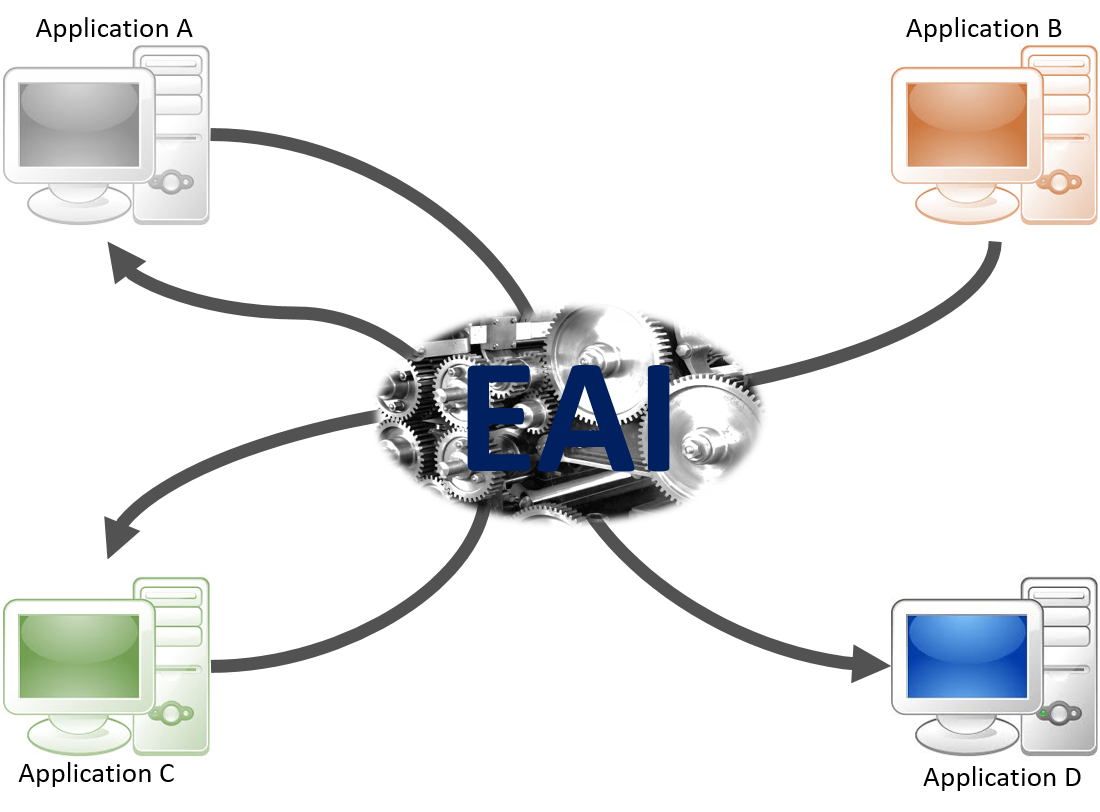
\includegraphics[width=10cm]{../img/eai_1.png}
				\caption{\label{intro_interop} L'EAI est un outil qui permet
				d'établir des routes entre applications métier.}
			\end{figure}
			Cloverleaf est un EAI dédié au monde hospitalier (il n'est cependant pas le
			seul).
			
			\paragraph{}% transfo de messages
			Les fonctions de l'EAI ne se résument pas au seul transport des données. Il
			est parfois utile de réaliser des actions sur les informations transmises
			d'une application à l'autre (figure \ref{interop_transfo}). Ces actions
			peuvent êtres par exemple~:\newline
			\begin{itemize}
			  \item de valider les informations transmises. Par exemple, l'EAI va
			  s'assurer que pour chaque donnée émise par une application de gestion des
			  prescriptions, le nom du patient est bien présent.
			  \item d'effectuer des transformations. L'application destinataire ne
			  gère pas forcément les mêmes formats de données que l'application émettrice
			  car, rappelons-le, les applications ne sont pas forcément conçues pour
			  fonctionner ensemble. L'EAI est ainsi capable de faire des conversions de
			  format de donnée.\newline
			\end{itemize}
			\begin{figure}[H]
				\centering
				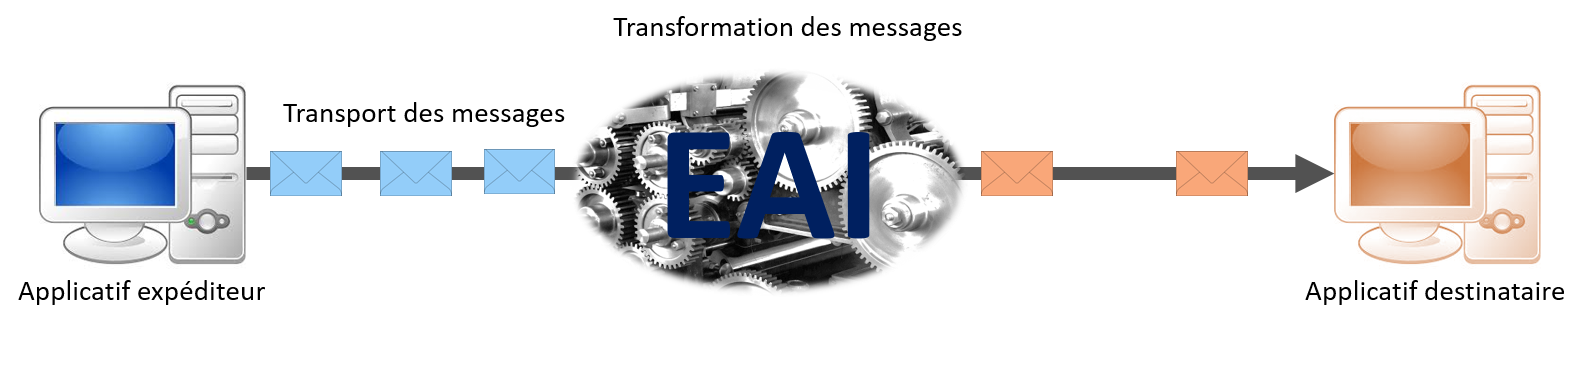
\includegraphics[width=15cm]{../img/eai_2.png}
				\caption{\label{interop_transfo} Un EAI peut effectuer des opérations sur
				les données qui transitent par lui.}
			\end{figure}
			
			\paragraph{}% Un peu de vocabulaire
 			Il existe un vocabulaire pour désigner les transferts de données entre
 			applications. Dans la suite, nous parlerons de~:
 			\begin{description}
 				\item[Flux] Les flux sont tout simplement les routes permettant de
 				connecter une application à une autre. Dans un système d'information hospitalier
 				(SIH), il y a donc autant de flux que de couple d'application. Il est
 				possible - et même courant - qu'une application soit reliée à plusieurs
 				autres.
 				\item[Message] Les données qui passent le long des flux, d'une application
 				à une autre, sont appelées messages. Les messages se présentent en général
 				sous la forme de texte hautement standardisé. Les messages sont émis par les
 				applicatifs métier dans un format donné. Il existe de nombreux formats
 				dont certains sont spécifiques au monde hospitalier. L'annexe 1 présente
 				quelques-uns des principaux formats utilisés (les formats HL7 et HPRIM).
 			\end{description}

		\subsubsection{Les flux de messages doivent être surveillés}
			\paragraph{}% Importance fonctionnelle de la supervision
			L'EAI est un outil complexe et dont le bon fonctionnement est essentiel. En
			effet, c'est tout le SI de l'hôpital qui repose en permanence sur lui. Si
			un disfonctionnement intervient, des pans entiers du
			service hospitalier risquent d'en pâtir, ce qui aura des conséquences sur le
			traitement des patients. Lorsqu'un disfonctionnement survient au niveau d'un
			flux, au point que celui-ci ne peut plus transmettre ses messages, on dit
			qu'il tombe en erreur.

			\paragraph{}% Exemple de cas de disfonctionnement
			Il existe différentes raisons pour lesquelles un flux peut tomber en erreur.
			La figure \ref{interop_erreur} expose les trois principales. La cause (1)
			évoquée sur le schéma, correspond à une erreur qui survient entre l'application source et l'EAI,
			c'est-à-dire lors du transfert du message de l'application à l'EAI. Une
			erreur de ce type peut avoir des causes variées. Il peut s'agir d'un problème
			au niveau du réseau qui transporte les messages (par exemple une coupure
			d'internet). Le cas (2) correspond à une erreur qui est levée
			lors du traitement du message par l'EAI. Il se peut que le contenu du
			message ne soit pas conforme à ce qu'attendait le script réalisant le
			traitement. Ce peut être par exemple le cas lorsqu'un utilisateur de
			logiciel métier fait un erreur de saisie et que cette erreur n'est pas
			relevée par le logiciel en question. Enfin, dans le cas (3), les messages
			s'accumulent à la sortie de l'EAI car la route entre l'EAI et l'application
			destinataire est bloquée, par exemple par une coupure momentanée du réseau.
			\newline
			\begin{figure}[H]
				\centering
				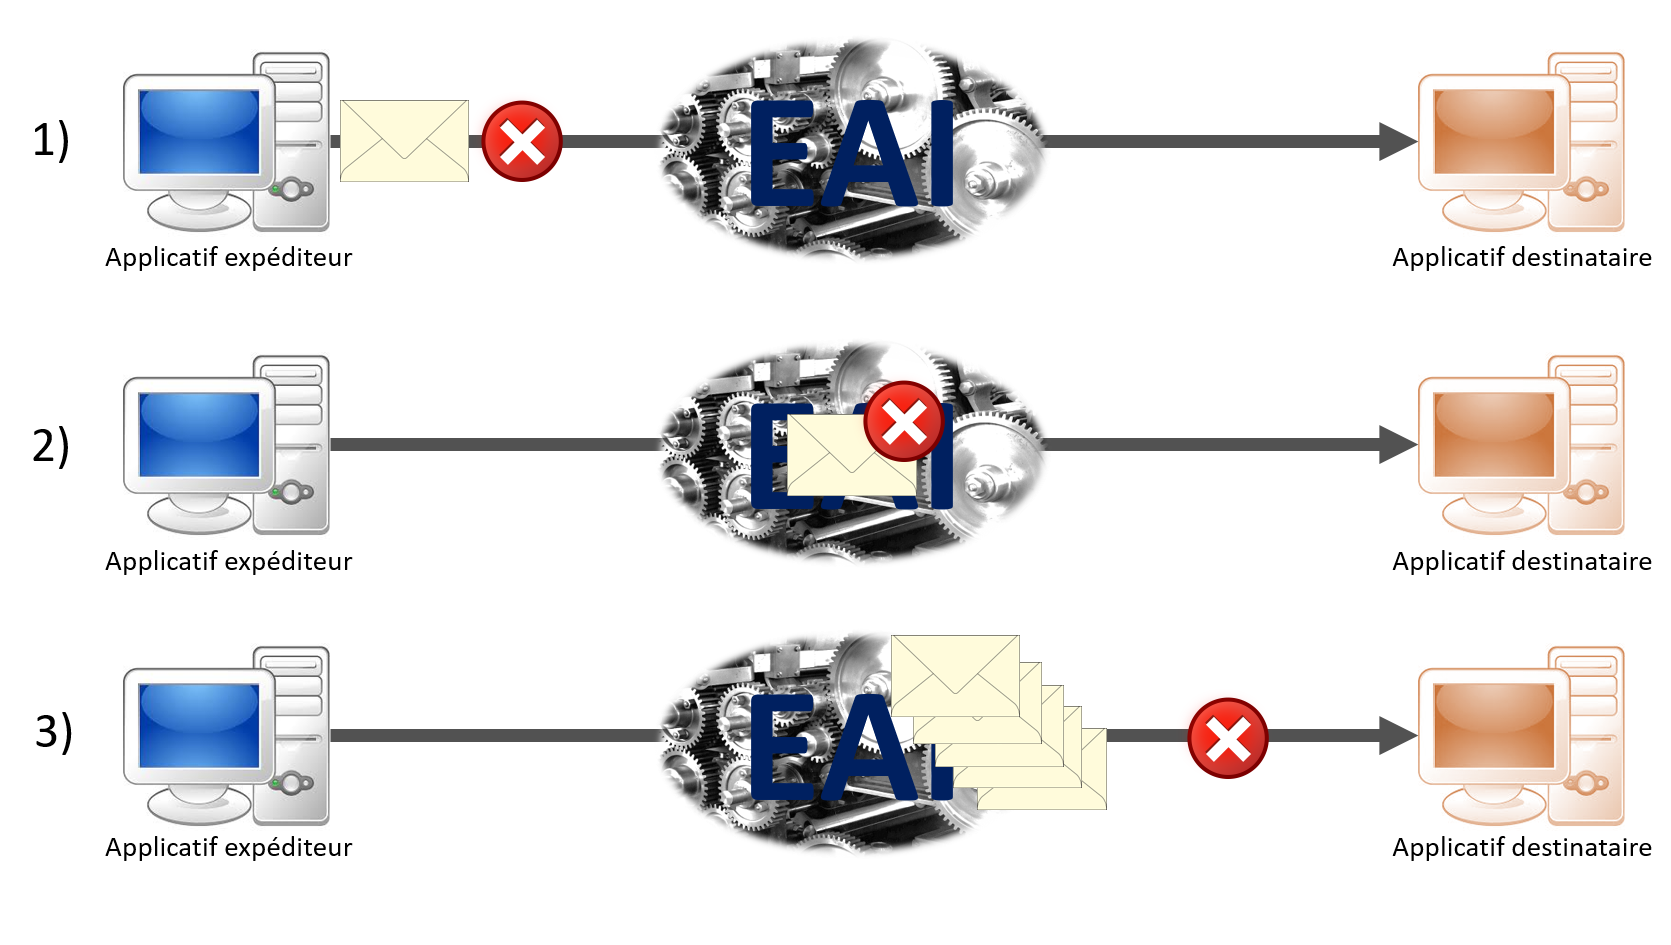
\includegraphics[width=15cm]{../img/error_1.png}
				\caption{\label{interop_erreur} De multiples causes d'erreurs peuvent
				stopper momentanément un flux de message.}
			\end{figure}
			
			\paragraph{}% Surveiller un flux c'est pas facile
			Ainsi, il est capital d'exercer une surveillance continue sur les différents
			flux, pour être certain que l'EAI assure bien ses fonctions et que les
			messages transitent correctement. Cette surveillance est ce que l'on appelle
			la supervision des flux. Cette tâche peut être assurée grâce à deux outils~:
			\begin{itemize}
			  \item L'environnement de développement intégré (IDE) de Cloverleaf. Cet
			  outil permet de contrôler tout l'EAI, c'est-à-dire aussi bien assurer la
			  supervision que de mettre en place de nouveaux flux. L'IDE est un outil
			  très complexe qui nécessite une formation spécialisée, ce que les
			  personnels des services informatiques des centres hospitaliers n'ont pas
			  forcément.
			  \item Les consoles de supervision.
			\end{itemize}
			
		\subsubsection{TrackCIS est un outil qui permet la supervision des flux}
			\paragraph{}% C'est quoi une console de supervision ?
			Une console de supervision permet d'assurer la surveillance
			de tout ou partie des flux gérés par l'EAI. Elle dispose d'un
			nombre limité de fonctionnalité par rapport à l'IDE mais se veut plus simple
			et plus rapide d'utilisation. Il existe actuellement pour Cloverleaf un
			certain nombre de consoles~:
			\begin{description}
				\item[Global Monitor] Cette console est développée par le même éditeur qui
				est à l'origine de Cloverleaf~: Infor. Global Monitor est un outil assez
				complexe, il est destiné à des personnes relativement rompues au
				fonctionnement de l'EAI.
				\item[EAI Supervision] Cet outil est développé par l'un des plus gros
				éditeurs de logiciels hospitalier français~: Maincare. Cette console ne
				permet cependant pas de gérer tous les flux, mais seulement ceux faisant
				intervenir des applications développées par Maincare.
				\item[TrackCIS] Cette console a été développée par Xperis. Elle est destinée
				à des utilisateur ne maîtrisant pas forcément l'EAI.
			\end{description}
			
			\paragraph{}% Les principales fonctionnalités
			Nous nous focaliserons dans la suite sur la console de supervision TrackCIS.
			En voici les principales fonctionnalités~:
			\begin{itemize}
			  \item Visualiser la liste des messages qui transitent dans le flux en temps
			  réel. L'utilisateur peut ainsi voir les données qui passent par l'EAI. Il
			  a accès à des informations sur ces messages comme leur date d'émission, ou
			  leur état. Ils peuvent par exemple voire si un message est en erreur, c'est
			  à dire s'il est bloqué quelque part dans l'EAI.
			  \item Pouvoir éditer et rejouer les messages. Lors d'une erreur, il peut
			  être utile pour la personne en charge de la supervision de pouvoir modifier
			  à la main le contenu du message. Ceci peut s'avérer utile quand l'erreur
			  est due à une erreur de saisie par l'utilisateur de l'application de
			  départ.
			  \item La rejoue de message. Une fois une erreur corrigée, l'utilisateur de
			  la console peut rejouer le message, c'est à dire le refaire passer dans
			  l'EAI de façon à ce qu'il rejoigne l'application destinatrice. La rejoue de
			  message peut également s'avérer utile lorsque les messages ne sont pas
			  correctement intégrés dans l'outil à leur sortie du flux. Une fois le
			  problème résolu au niveau de l'application de sortie concernée, il faut
			  rejouer les messages pour les refaire transiter correctement.
			\end{itemize}
		
		\paragraph{}% Résumé de la partie 1.1
		Nous avons vu dans cette première partie que l'EAI est une solution au
		problème de l'interopérabilité en établissant des flux de données entre
		applications métier. Nous avons souligné le fait que la surveillance (la
		supervision) continue des flux est indispensable au bon fonctionnement de
		l'EAI et, par extension, de tout le SI. Enfin, TrackCIS est un outil qui
		permet de rendre la supervision plus simple et plus rapide.\newline
		Dans la suite nous découvrirons les problématiques inhérentes à cet outil.
		
	\subsection{TrackCIS est au cœur d'une problématique commerciale pour Xperis}
		\paragraph{}
		Précédemment nous avons établi les bases des problématiques d'interopérabilité
		des établissements hospitaliers. Xperis est une entreprise qui propose
		d'accompagner ces derniers dans la mise en place et le maintien de Cloverleaf.
		Cette société se trouve à l'intermédiaire entre de nombreux acteurs que nous
		allons présenter.
		
		\subsubsection{Cloverleaf est un EAI du secteur de la santé}
			\paragraph{Les établissements hospitaliers~:}% panorama du monde hospitalier
			Le premier parti prenant est l'utilisateur final de
			Cloverleaf c'est-à-dire l'ensemble des établissements hospitaliers
			français.
			Au 31 décembre 2014, on dénombrait en France 3 111 établissements hospitaliers,
			dont 1 416 établissements publics. Ces derniers sont répartis en trois
			catégories \citep{drees_panoramas_2016}~:
			\begin{itemize}
				\item 182 centres hospitaliers régionaux (CHR)~: ils dispensent des soins 
				spécialisés à la population de la région,
				\item 973 centres hospitaliers (CH)~: ils assurent les soins médicaux, 
				chirurgie et prise en charge des personnes âgées,
				\item 97 centres hospitaliers psychiatriques,
				\item 164 établissements de soins longue durée.
			\end{itemize}
			Les hôpitaux privés sont répartis en deux catégories~:
			\begin{itemize}
				\item 1 012 établissements privés à but lucratif,
				\item 683 établissements à but non lucratif, dont 21 centre de lutte contre 
				le cancer.
			\end{itemize}
			
			\paragraph{Infor~:}
			C'est la société américaine qui développe l'EAI Cloverleaf. Infor distribue
			son EAI dans de nombreux pays du monde par l'intermédiaire de sociétés
			telles que Xperis.
			
			\paragraph{Les éditeurs~:}
			Les éditeurs de logiciels médicaux sont de grosses sociétés dont la
			croissance est assurée par de nombreuses fusions et acquisitions. Ainsi ils
			proposent des solutions logicielles très diverses, car initialement
			développées par des sociétés différentes. Ce sont ces entreprises qui
			achètent l'EAI et le mettent en place chez leurs clients, les hôpitaux. Parmi
			les principaux éditeurs du monde hospitalier on trouve~:
			\begin{itemize}
				\item Maincare
				\item Le SIB (Syndicat Interhospitalier de Bretagne)
				\item Le MIPIH (Midi Picardi Informatique Hospitalière)
			\end{itemize}
			
		\subsubsection{Xperis cherche à établir des liens directs avec les hôpitaux}
			\paragraph{Xperis~:}
			Xperis est le seul distributeur (ou master distributeur) de la solution
			Cloverleaf en France. La société est basée à Bordeaux, compte une dizaine de
			salariés et est l'intermédiaire entre Infor et les éditeurs.
			Même si ces derniers sont les principaux clients de l'entreprise,
			l'entreprise cherche actuellement à établir des relations commerciales
			directes avec les établissements hospitaliers.\newline
			La figure \ref{xperis_secteur} résume les interactions qui existent entre
			tous ces acteurs.
			\begin{figure}[H]% Position d'Xperis dans le secteur de la santé
				\centering
				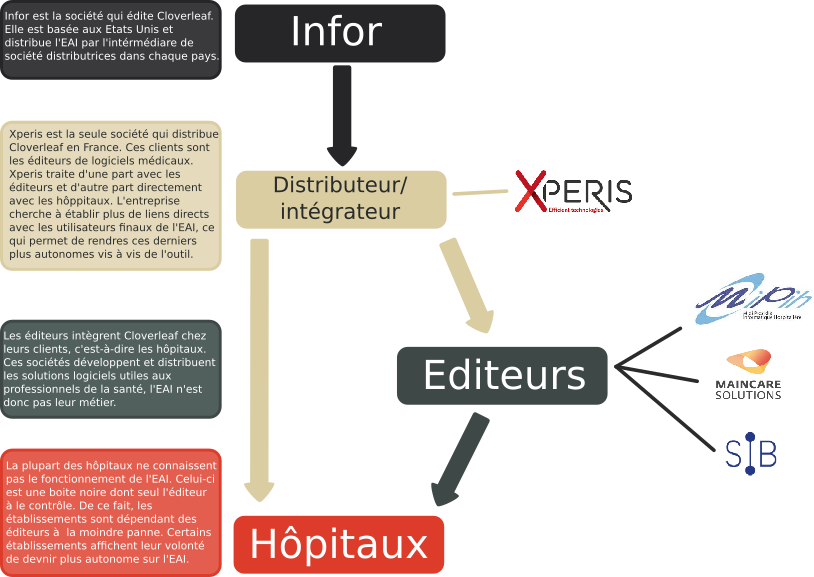
\includegraphics[width=17cm]{../img/xperis_secteur.png}
				\caption{\label{xperis_secteur} Xperis est l'intermédiaire entre Info et
				les éditeurs français.}
			\end{figure}
			
			\paragraph{}% regroupement des hôpitaux en GHT
			Depuis 2016, une directive nationale prévoit le regroupement des établissements de 
			santé publics français en groupements hospitaliers de territoire (GHT) 
			\citep{valls_decret_2016}. Dans le cadre d'un GHT, les établissements doivent mettre 
			en commun leur système d'informations et doivent utiliser les mêmes logiciels et 
			applicatifs métiers. Le décret prévoit en outre la création de 135 GHT  
			\citep{touraine_marisol_2016}. Ceci risque d'impacter l'activité d'Xperis dans la 
			mesure où, lorsque les GHT seront formés, les outils d'interopérabilités 
			(les EAI) seront également mutualisés.
			
			\paragraph{}% La stratégie d'Xperis face à ces challenges
			Pour faire face à ces challenges, l'entreprise cherche de plus 
			en plus à traiter directement avec les établissements hospitaliers. TrackCIS
			contribue à cela puisqu'il s'agit d'un outil développé en interne et
			distribué directement aux hôpitaux.
			
		\subsubsection{Un outil qui se vend mal et qui est peu utilisé}
			\paragraph{}% L'objectif initial du projet TrackCIS
			Comparativement aux autres consoles de supervision, TrackCIS se veut plus
			simple et plus ergonomique. Initialement, le public visé était les
			utilisateurs métier, c'est-à-dire des personnes ne travaillant pas dans le
			milieu informatique comme par exemple des infirmiers ou des pharmaciens. Ces
			personnes, ou référents métiers, sont des utilisateurs d'applications
			médicales. Le projet de TrackCIS avait pour objectif de confier une partie de
			la supervision de l'EAI à ces personnes, sur les flux qui les intéressaient.
			Ainsi, si un utilisateur rencontre un problème lié à l'interopérabilité avec
			une des applications (par exemple un patient enregistré à l'accueil mais dont
			les informations ne sont pas présentent dans le logiciel de gestion des
			dossiers médicaux), il peut se tourner vers le référent métier plutôt que
			vers le service informatique. Ce type de démarche permettrait de supprimer
			des intermédiaires et donc de diminuer le temps de résolution des problèmes.
			
			\paragraph{}% Le problème actuel avec cet outil
			Mais le projet TrackCIS n'a pas pris et même si quelques consoles ont été
			vendues, peu de CH l'utilise pleinement. Les raisons à cela peuvent être
			multiples et relativement méconnues d'Xperis. L'une d'elles est que la
			console n'est pas vendue pré-paramétrée et que c'est au CH de faire ce
			paramétrage.
			Celui-ci peut représenter une charge assez lourde. Une autre raison serait
			que les référents métiers ne soient pas encore mis en place dans les
			hôpitaux.
			
	% Résumé de la partie 1.2
	\paragraph{}
	Nous avons vu qu'Xperis est confronté à un certain nombre de problématiques
	commerciales. L'entreprise à une vraie volonté de traiter en direct avec les
	hôpitaux pour gagner en indépendance vis à vis des éditeurs. TrackCIS entre
	dans cette stratégie mais a du mal à se faire une place parmi les
	clients.\newline
	L'ensemble de ces problématiques constitue le socle de notre travail.
	
	\subsection{Vers une nouvelle version de TrackCIS}
		\paragraph{}% problème => solution commerciale ou solution fonctionnelle
		Le problème que pose TrackCIS soulève une question~: pourquoi cet outil ne se
		vend-il pas ? La réponse à cette question, loin d'être triviale, pourrait
		être de deux natures: une solution commerciale et une solution fonctionnelle.
		\begin{description}
			\item[La solution commerciale~: ] Nous faisons ici l'hypothèse que la cause
			au fait que TrackCIS ne se vende pas est commerciale. Ceci pouvant impliquer
			plusieurs choses comme le fait que~:
			\begin{itemize}
			  \item les clients n'ont pas réellement besoin d'un outil tel que TrackCIS.
			  Il existe en effet d'autres outils de supervision pour Cloverleaf, comme
			  par exemple l'outil Global Monitore, dont nous reparlerons un peu plus
			  loin, ou encore EAI Supervision.
			  \item les utilisateurs de TrackCIS n'existent pas. Cet outil a été
			  développé pour des personnes non initiées à Cloverleaf mais qui pour qui
			  il serait intéressant de superviser quelques flux.
			  Or il est tout à fait possible que ce type de personne n'existe pas ou pas
			  encore dans les hôpitaux.
			  \item la communication ou le démarchage autour de TrackCIS est insuffisant
			  ou non adapté.
			\end{itemize}
			\item[La solution fonctionnelle~: ] Cette fois-ci notre hypothèse est que
			TrackCIS ne se vend pas car il lui manque des fonctionnalités indispensables
			à ses utilisateurs.
		\end{description}
		
		\subsubsection{Comprendre les utilisateurs et leurs besoins}
			\paragraph{}% Nous ne traitons que de la solution fonctionnelle
			De ces deux solutions à la problématique soulevée par TrackCIS (commerciale
			ou fonctionnelle), nous prenons le parti de n'en traiter qu'une, la
			seconde.\newline
			L'objectif assumé de ce mémoire est de traiter de l'amélioration
			fonctionnelle et technique d'un outil tel que TrackCIS. Notre objectif est de
			chercher à connaitre
			
			\paragraph{}% Les anciennes specs ne permettent pas de bien comprendre le besoin des utilisaturs
			Comme nous l'avons vu jusque-là, les raisons du manque de
			popularité de TrackCIS auprès des clients d'Xperis sont multiples et
			méconnues. L'une des principales questions que soulève ce problème est de
			savoir qui sont les utilisateurs de TrackCIS. Actuellement il n'y a que très
			peu de réels utilisateurs. Il s'agit de comprendre dans un premier temps quel
			public est susceptible d'utiliser au quotidien un tel outil. Notre objectif
			est de comprendre comment réadapter cet outil au besoin des utilisateurs, il
			nous faut donc comprendre qui ils sont. Il nous faut également comprendre
			leurs besoins et traduire ceux-ci en fonctionnalités implémentables dans
			l'outil. Voici donc le principal point de départ de notre travail.
			
		\subsubsection{Un module statistique lié aux évolutions de Cloverleaf}
			\paragraph{}% Volonté de développer un module stat
			A ce stade, les améliorations à apporter à TrackCIS nous sont encore
			inconnues. Cependant, l'une d'elles pourrait consister en l'implémentation
			d'un module d'affichage de statistiques. Xperis affiche une volonté forte de
			développer un tel module qui apporterait un double avantage à l'outil~:
			\begin{itemize}
			  \item Une innovation. En effet, la possibilité de récupérer des
			  statistiques de Cloverleaf est une fonctionnalité récente de l'EAI que peu
			  de consoles de supervision utilisent pleinement à ce jour. Un module
			  statistique apporterait à l'utilisateur une expérience nouvelle sur la
			  supervision de l'EAI, et donc un rôle nouveau à TrackCIS.
			  \item De plus, les statistiques vont dans le sens de la philosophie de
			  TrackCIS et des consoles de supervision en général~: avoir une vue
			  d'ensemble instantanée de l'état d'un flux. L'affichage de telles données
			  pourrait apporter une nouvelle manière de superviser à l'utilisateur.
			\end{itemize}
			
			\paragraph{}
			Ce module statistique représente l'axe principal du projet développé ici. Si,
			dans la suite nous nous consacrerons à comprendre comment, d'une manière
			générale, améliorer TrackCIS, seul le module statistique sera implémenté
			techniquement à l'outil. Les autres fonctionnalités pourront l'être dans les
			travaux qui feront suite à ce mémoire.
			
		\subsubsection{Méthodologie générale du projet}
			\paragraph{}% Résumé des problèms soulevés
			Nous avons constaté dans les parties précédentes plusieurs problématiques
			inhérentes à TrackCIS. Nous avons également pris le parti de tenter de
			répondre à ces problématiques selon une logique fonctionnelle, de qui
			implique de développer de nouvelles fonctionnalités sur cet outil.
			
			\paragraph{}% Cadrage de notre travail
			Avant d'exposer la méthodologie suivie dans ce projet, fixons les limites de
			ce projet. Nous ne nous intéresserons ici qu'au développement d'un
			module d'affichage de statistiques dans TrackCIS. Les raisons à ce choix sont
			:
			\begin{itemize}
			  \item Le développement d'un tel module est un objectif prioritaire pour
			  Xperis concernant TrackCIS.
			  \item La possibilité de récupérer des statistiques sur le fonctionnement de
			  Cloverleaf est une fonctionnalité nouvelle de l'EAI. Aucune console de
			  supervision n'en n'a pour l'instant totalement exploité les possibilités.
			  \item De ce fait, ce nouveau module peut apporter un facteur de
			  différentiation notable à TrackCIS par rapport aux autres consoles.
			  \item Ceci pourrait apporter une solution à la problématique commerciale
			  de TrackCIS, à savoir le fait qu'il s'en vend peu.
			\end{itemize}
			Cependant, l'implémentation de ce seul module statistique n'apporterait une
			réponse fonctionnelle complète. En effet, les besoins des utilisateurs sont à
			ce jour mal connus par l'entreprise. La typologie même de ces utilisateurs
			est aujourd'hui difficile à définir.\newline
			Notre objectif est donc le suivant~:\newline
			Contribuer à l'amélioration de TrackCIS par l'implémentation d'un module de
			statistiques et par une analyse des besoins dans le but de propositions
			d'autres axes d'amélioration.

			\paragraph{}% Méthodologie générale + présentation de l'approche
			% fonctions -> comportements -> structure de Xavier Blanc
			Pour ce faire, nous procéderons en trois grandes étapes~: l'analyse du
			besoin, la conception d'une solution et son développement. Au cours de
			chacune de ces étapes nous serons amenés à modéliser différents aspects de
			l'application~:
			\begin{itemize}
			  \item Modélisation des fonctions de l'application. Nous établirons une
			  liste des fonctionnalités qui permettra d'aboutir à la solution finale.
			  Nous établirons cette liste à partir des besoins des utilisateurs.
			  \item Modélisation des comportements de l'application et des utilisateurs.
			  Nous imaginerons des scénarios d'utilisation pour les différentes
			  fonctionnalités à développer.
			  \item Modélisation de la structure de l'application. Il s'agira de définir
			  les moyens techniques ainsi que l'architecture du module à développer.
			\end{itemize}
			
			\paragraph{}% Détail pour la phase d'analyse du besoin
			Les deux parties suivantes vont présenter la mise en oeuvre d'une
			méthodologie qui nous permettra d'une part de connaître les besoins des
			utilisateurs et comment les satisfaire avec TrackCIS, et d'autre part la
			mise en pratique de ces améliorations au travers d'un nouveau module.
			
			
			
	\chapter{Phase d'analyse : des besoins aux fonctionnalités}
	\paragraph{}
	Dans la partie précédente nous avons vu ce qu'est un EAI et les enjeux de la
	supervision. Nous avons vu que TrackCIS est une console de supervision et
	notre projet vise à l'améliorer.
	Dans cette deuxième partie, nous chercherons à comprendre les besoins des
	utilisateurs de consoles de supervision et nous les traduirons en
	fonctionnalités implémentables dans TrackCIS.
	
	\subsection{L'enquête permet une meilleure compréhension des besoins des utilisateurs}
		\paragraph{}
		Un besoin est formulé par le destinataire d'une application, l'utilisateur. Il
		peut l'être explicitement ou implicitement. Dans le cas qui nous intéresse il
		nous importe de comprendre les besoins des utilisateurs potentiels de
		TrackCIS. De plus, pour véritablement comprendre ces besoins, nous devons
		aussi savoir qui sont les utilisateurs. L'enquête nous permettra d'obtenir ces
		informations.
		
		\subsubsection{Élaboration d'un questionnaire d'enquête et conduite des entretiens}
			\paragraph{}% Les objectifs de l'enquêtes
			L'enquête poursuit deux objectifs :
			\begin{itemize}
			  \item D’une part nous souhaitons pouvoir établir une liste de besoins.
			  \item D’autre part, cette enquête sera l’occasion de comprendre un peu
			  mieux comment sont organisés les DSIO (direction des services informatique
			  et de l’organisation) des établissements hospitaliers, ainsi que de faie
			  une typologie des utilisateurs de consoles de supervision.
			\end{itemize}
			
			\paragraph{}% Les grands thèmes abordés
			Pour répondre à ces deux objectif, le questionnaire d’enquête doit être le
			plus générale possible et les questions ouvertes. Ainsi, nous proposons le
			plan d'entretien suivant :
			\begin{itemize}
			  \item[1) Identification de la personne, exploration du contexte] . Cette
			  partie aura pour but de nous aider à comprendre comment est organisé le
			  service et qui est notre interlocuteur.
			  \item[2) Utilisations et utilisateurs de Cloverleaf et problématique de la
			  supervision des flux] . Dans cette partie nous poserons des questions sur
			  la manière dont est utilisé Cloverleaf et par qui ainsi que les personnes
			  qui sont en charge de la supervision.
			  \item[3) Attentes par rapport aux consoles de supervision] Cette partie,
			  beaucoup plus abstraite, servira à comprendre ce qu’est la supervision
			  pour les utilisateurs de consoles et quels sont les attentes des
			  utilisateurs sur les consoles de supervision.
			  \item[4) Les consoles actuelles] Ces questions viseront à explorer ce que
			  les utilisateurs utilisent le plus dans les outils existant, quels sont
			  les manques et les améliorations qu’ils proposent. Cette partie explorera
			  également les propositions des utilisateurs concernant un future module
			  statistique.
			\end{itemize}
			
			\paragraph{}% Conduite des entretiens
			Les entretiens sont conduit de manière semi-directive par téléphone ou en
			face à face quand cela est possible.
			Les questions présentent dans le guide d'entretien ne sont que des guides
			pour orienter la discussion, c’est pourquoi elles sont les plus ouvertes possible.\newline
			Le questionnaire a vocation à évoluer d’un entretien à un autre : des
			questions peuvent être modifiées, supprimées ou ajoutées de façon à obtenir
			des informations de plus en plus pertinentes (l'annexe 2 présente la dernière
			version du guide d'entretien). Chaque entretien donne lieu à un compte-rendu
			détaillé dont la structure reprend la trame du questionnaire.
			
			\paragraph{}% Les principes de l'étude qualitative
			Il s'agit d'une étude qualitative. Contrairement aux études quantitatives qui
			permettent de récolter des données repérsentatives d'une population donnée,
			dans une étude qualitative nous ne cherchons pas à interroger le plus de
			personnes possible. Les entretients sont basés sur des question ouverte et
			durent en général plus longtemp que dans des enquêtes quantitatives, une
			trentaine de minute dans notre cas.
			L'objetcif d'une telle étude est de faire ressortir la diversité des
			comportement. Ici, il s'agit entre autre de mettre en avant les différentes
			utilisations possibles des consoles de supervision et ses utilisateurs.
			
			\paragraph{}% Choix de la population interrogée
			Un panel de 5 établissements hospitaliers est interrogé. Tous ces
			établissements sont des clients d’Xperis :
			\begin{itemize}
			  \item Tour
			  \item Toulouse
			  \item Rouen
			  \item Brest
			  \item Metz
			\end{itemize}
			
			\paragraph{}% Méthodes d'analyse des résultat
			A l'issue des enquêtes nous procédons à l'analyse des résultats. Après une
			rapide relecture de tous les comptes rendu d'entretien, nous établissons une
			listes des grands thèmes qui ont été abordés durant les discussion.
			On classe ensuites chaque information collectée dans l'un de ces
			thèmes.\newline Les grand thèmes en question sont les suivants :
			\begin{itemize}
			  \item[- grand thème 1] L’organisation des services informatique dans les
			  hôpitaux,
			  \item[- grand thème 2] Les types d’utilisateurs de TrackCIS,
			  \item[- grand thème 3] Les types d’utilisations de TrackCIS,
			  \item[- grand thème 4] Les attentes par rapport aux consoles de supervision
			  et la réponse des outils actuels à ces attentes,
			  \item[- grand thème 5] Les fonctionnalités manquant aux consoles de
			  supervisions actuelles,
			  \item[- grand thème 6] Les statistiques sur les flux.
			\end{itemize}
			Dans la suite de cette partie nous entrerons dans le détail des informations
			collectées pour chacun de ces grand thèmes.
			
		\subsubsection{La supervision fait partie du processus de résolution des
		anomalies}
			\paragraph{}% Présentation
			Nous analysons ici l'organisation interne des services liées à
			l'interopérabilité dans les hôpitaux. Nous verons ensuite quelles sont les
			pratiques liées à la supervision (autrement dit, nous détaillerons les
			grands thèmes 1 et 3).
			
			\paragraph{}% L'organisation des DSIO
			Les services informatiques ont des structures très variables selon les
			établissements. Cependant, il existe dans tous les cas observés au moins un
			département consacré à l’interopérabilité. Ce département peut se subdiviser
			en deux pôles :
			\begin{itemize}
			  \item Un pôle intégration,
			  \item Un pôle exploitation
			\end{itemize}
			\textbf{Le pôle intégration} prend en charge la mise en place de nouveaux
			flux et du bon fonctionnement de l’EAI en général. Son niveau de compétence sur
			Cloverleaf est élevé. Ce type de pôle existe dans des établissements
			relativement autonomes vis-à-vis des éditeurs de logiciels. Le pôle
			intégration se compose généralement de 2 à 3 personnes. Les outils utilisés
			sont principalement l’IDE, et des consoles de supervision telles que EAI
			Supervision ou Global Monitor.\newline
			\textbf{Le pôle exploitation} a en charge la supervision des flux. Le niveau
			de maîtrise de Cloverleaf y est plus faible. Les outils utilisés sont en
			général les différentes consoles de supervision,
			mais rarement l’IDE, trop complexe pour ce type d’utilisateur.\newline
			Les deux pôles peuvent cohabiter au sein d’un même établissement. Certains,
			comme le CHU de Metz, n’ont qu’un pôle exploitation, la mise en place des
			flux étant assuré par un autre département (en l’occurrence, le département
			en charge de l’urbanisation du SI). D’autres établissements, beaucoup plus
			dépendants des éditeurs, ne s’occupent pas de la mise en place des flux ni
			du fonctionnement de l’EAI, mais seulement de la supervision. C’est par
			exemple le cas du CHU de Châtellerault.\newline
			La figure \ref{orga_interop} résume les différents niveaux de gestion de
			l’interopérabilité au sein d’un hôpital. Les niveaux correspondent au degré
			de responsabilité vis à vis de l'interopérabilité. Plus un niveau est élevé,
			plus les impactes des décisions prises à ce niveaux seront fort sur le SI. Un
			pôle exploitation se situe au niveau le plus bas tandis qu’un pôle
			intégration peut se situer au niveau 2 ou 3. Le niveau le plus haut est en
			général assuré par un département urbanisation, en charge de la définition
			de la politique de tout le SI.
			% Niveau de responsabilité pour l'interop dans le SI
			\begin{figure}[H]
				\centering
				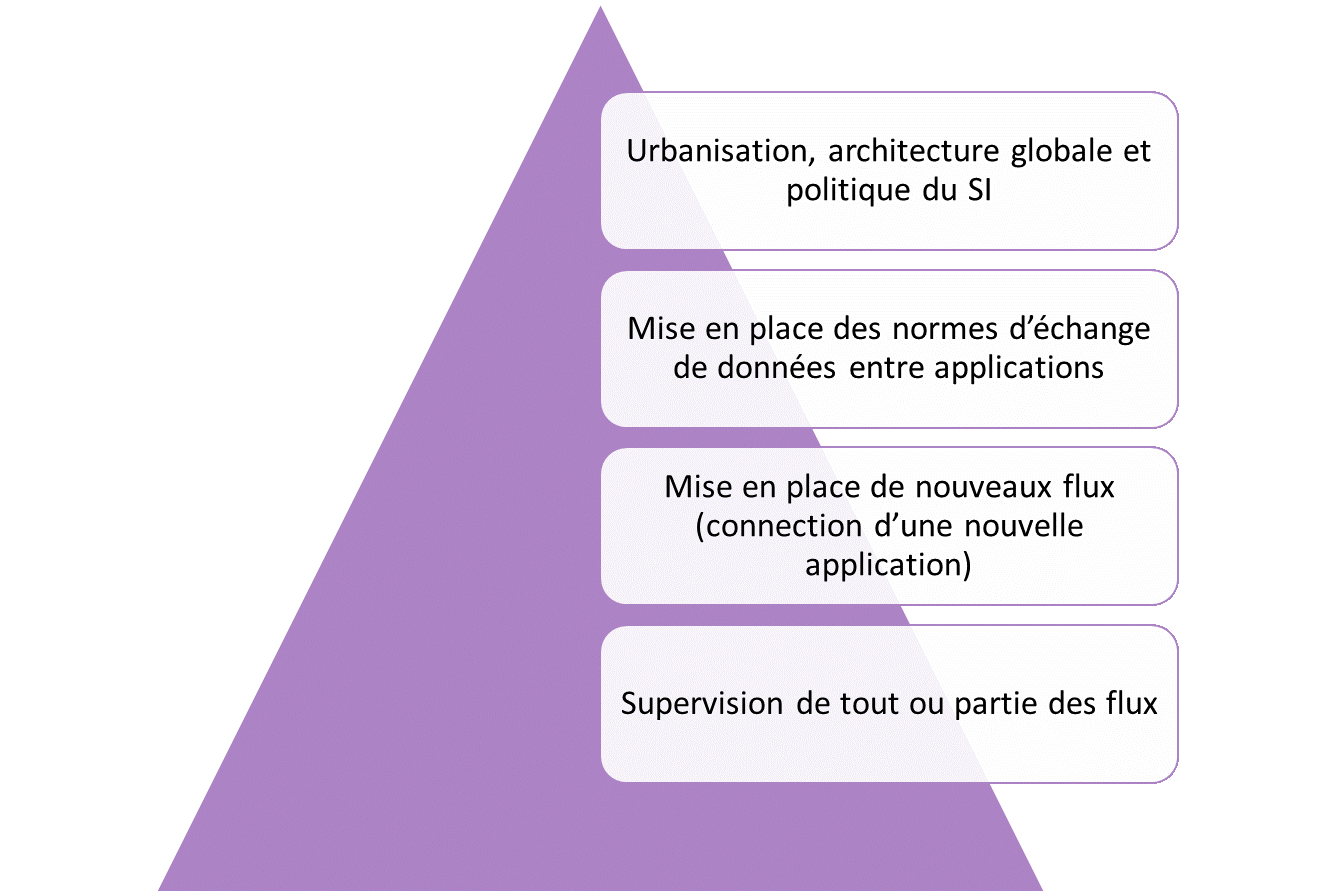
\includegraphics[width=8cm]{../img/si_1.png}
				\caption{\label{orga_interop} Les différents niveaux de responsabilité
				autour de la gestion de l'interopérabilité.}
			\end{figure}
			
			\paragraph{}% Diversité des pratiques
			L’ensemble des outils liés à Cloverleaf (IDE et consoles de supervision)
			sont utilisés pour la supervision des flux. Les utilisateurs les plus
			aguerris sur Cloverleaf utilisent l’IDE, notamment à une fonctionnalité,
			nomée \textit{status}, qui donnes accès à des données statistiques sur un
			thread ou un process à un instant t. Pour détecter les problèmes,
			l’utilisateur se fie principalement à la date et heure de dernière écriture
			d’un message sur le flux. Si rien n’a été écrit depuis un certain temps, c’est que
			le flux est bloqué et que les messages ne passent plus. Ce type d’utilisateur est
			généralement en charge de la résolution des problèmes les plus complexes.
			Pour cela, il a parfois recours à des fonctionnalité avencées comme la
			consultation de la base de donnée d'erreur (ou \textit{error database}) ou
			à base de données contenant les messages pour comprendre l’origine de
			l’erreur.\\
			Du côté des consoles de supervision, les usages qui sont ressortis sont :
			\begin{itemize}
			  \item Visualiser l’état des flux (si les threads et process sont bien en
			  marche),
			  \item Affichage sur écran géant,
			  \item Rechercher un message en particulier, ou un certain type de
			  messages. Par exemple, tous les messages concernant un patient donné,
			  \item Visualiser les messages en erreur,
			  \item Supervision en mode lecture seule : vérifier que les messages
			  passent bien et connaître l’origine des erreurs,
			  \item Explorer le contenu des messages pour diagnostiquer une erreur,
			  \item Réaliser des tests lors de la mise en place de flux (usage repéré
			  uniquement au CHU de Toulouse),
			  \item Editer le contenu des messages en cas d’erreur,
			  \item Rejouer des messages après les avoir édités,
			  \item Pour les flux Maincare et EAI Supervision, s’assurer que les
			  messages sont bien intégrés dans les applications de destination,
			  \item Restreindre l’utilisation de certaines fonctionnalités pour par
			  exemple confier les outils à des personnes d’astreintes ou des personnes
			  métier,
			  \item Comparer le contenu d’un message entre son entrée dans un flux et
			  sa sortie. Cet usage n’a été référencé que pour EAI Supervision,
			  \item Paramétrer l’outil : création de colonnes, attribution des droits…
			\end{itemize}
			\paragraph{}
			Cette liste nous permet de connaître les principales utilisations des
			consoles de supervision (figure \ref{usage_consoles}). L’utilisation la plus
			simple est la visualisation : voir les messages qui passent et pouvoir détecter rapidement
			les erreurs. Une fois les erreurs détectées, l’utilisateur cherche à
			comprendre ce qui les a causées. Pour cela, il peut être suffisant de
			regarder le contenu du message pour en repérer les anomalies, ou bien aller
			dans l’error database. Une fois la cause de l’erreur bien établie, vient une
			phase de correction. Celle-ci peut se faire par édition du contenu du
			message et par rejoue, dans les cas les plus simples. Comme c’est le cas
			pour le CHU de Toulouse, la console peut être utilisée pour effectuer des
			tests lors de la mise en place de nouveaux flux. C’est-à-dire vérifier que
			les messages passent correctement d’une application à une autre. Enfin, les
			utilisateurs les plus avertis ont en charge l’administration de la console,
			c’est-à-dire son paramétrage (attribution des droits de consultation et
			d’action aux utilisateurs, paramétrage des données affichées\ldots). Ce rôle
			revient généralement au pôle intégration, aux éditeurs ou à Xperis. On
			remarque que, dans le cas de TrackCIS, le paramétrage de la console est un
			facteur limitant à son utilisation en production.
			\begin{figure}[H]% Niveau de responsabilité pour l'interop dans le SI
				\centering
				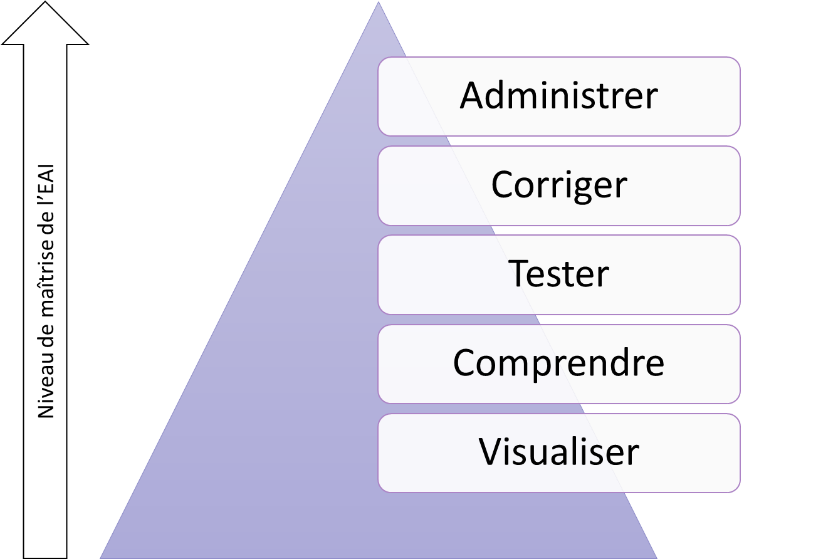
\includegraphics[width=10cm]{../img/usage_1.png}
				\caption{\label{usage_consoles} Les différents d'utilisation des consoles de
				supervision.}
			\end{figure}
			
			\paragraph{}
			En résumé, nous pouvons définir la supervision d'un flux comme :
			\begin{itemize}
			  \item Détecter en un coup d’œil la présence d’anomalies telles que :
			  	\begin{itemize}
			  	  \item Des erreurs,
			  	  \item Des ralentissements,
			  	  \item Des blocages
		  	    \end{itemize}
			  \item Pouvoir expliquer, même partiellement ces anomalies,
			  \item Et éventuellement pouvoir agir dessus dans le but de les corriger,
			  par exemple en rejouant un message qui n’est pas passé à cause d’un
			  problème momentané de la connexion. Selon deux des 5 personnes interrogées,
			  le but premier d'une console de supervision n'est cependant pas la
			  correction de anomalie, mais uniquement leur détection.
			\end{itemize}
			
		\subsubsection{Une grande diversité des utilisateurs des consoles de
		supervision}
			\paragraph{}% Présentation
			Nous savons maintenant comment à lieux la superision d'un flux dans la
			pratique et nous connaissons un peu mieux l'organisation en place dans les
			centres hospitaliers. Nous présenterons ici la typologie des utilisateur qui
			est ressortie de l'étude, ce qui correspond au grand thème 2.
			
			\paragraph{}% Les utilisateurs
			La typologie des utilisateurs découle du schéma d’organisation des services
			informatiques vu préciédemment (figure \ref{orga_interop}. On retrouve les
			deux niveaux que sont l’intégration et l’exploitation en plus d’un troisième
			niveau : le niveau métier. Le tableau \ref{type_utilisateurs} propose une
			description des 4 grands profils d’utilisateurs de consoles de supervision que l’étude a dégagée.
			\begin{table}[H]
				\centering
				\begin{tabular}{| p{3cm} | p{4,5cm} | p{4,5cm} | p{4,5cm} |} %Exemples des
				% principaux logiciels métier
					\hline
						\thead{Utilisateur}
						&\thead{Niveau de maitrise}
						&\thead{Outils utilisés}
						&\thead{Rôles}
						\\
					\hline
						Responsable d'intégration
						&
						Bon niveau de maîtrise de Cloverleaf.
						&
						Tous les outils (l'IDE, EAI Supervision, Global Monitor et TrackCIS)
						&
						Mise en place de nouveaux flux, résolution des problèmes complexes.
						\\
					\hline
						Responsable d'exploitation
						&
						Connaissances et formation de base sur l’EAI.
						&
						Consoles de superivision (EAI Supervision, Global Monitor et TrackCIS)
						&
						Surveillance, correction des erreurs simples (erreurs de contenus de
						messages), remonte les erreurs plus complexes
						\\
					\hline
						Personne d'astreinte
						&
						Il s'agit en général d'informaticiens mais non spécialisés et non formés
						sur Cloverleaf.
						&
						Consoles de supervision simples d'utilisations telles que TrackCIS ou
						Global Monitor.
						&
						Surveillance de quelques flux et éventuellement correction des erreurs les
						plus simples.
						\\
					\hline
						Référent applicatif
						&
						Pas ou peu de connaissance sur le fonctionnement de Cloverleaf. Il s'agit
						malgré tout de profils informaticiens.
						&
						Des consoles de supervision simple d'utilisation telle que TrackCIS.
						&
						Surveiller les flux concernant une application dont ils ont la charge. Les
						référents applicatifs existent déjà dans les hôptitaux, mais ils ne
						s'occupe pas de l'interopérabilité.
						\\
					\hline
						Référent métier
						&
						Pas de connaissances sur le fonctionnement de l’EAI. Typiquement il s'agit
						de personnel médical (infirmière, pharmacien\ldots) ou administratif.
						&
						Des consoles de supervision simple d'utilisation telle que TrackCIS.
						&
						Surveillance et éventuellement correction des erreurs simples. Ce type
						d'utilisateur n'existe pas encore dans les hôpitaux. Cependant, 3 des 5
						établissements interrogés disent avoir la volonté de mettre en place ce
						type d'utilisateur.
						\\
					\hline
				\end{tabular}
				\caption{\label{type_utilisateurs} Typologie des utilisateur dégagée par
				l'enquêtes.}
			\end{table}
			Ces différents acteurs coopèrent ensemble pour la résolution de problème,
			comme le résume la figure \ref{resolution_pbs}. Ce processus fait intervenir
			beaucoup d’intermédiaires ce qui pose problème à la fois aux utilisateurs métiers,
			car la résolution de problème prend du temps, et au services informatiques
			(notamment les pôles intégration et exploitation) car ils se retrouvent à
			devoir régler quotidiennement des problèmes parfois simple (comme des
			erreurs de saisie). Ceci justifie la volonté de certains établissements,
			comme le CHU de Toulouse, de donner accès à des utilisateurs métiers
			d’applications la possibilité de corriger les erreurs les plus simples
			(comme les erreurs de saisie).
			\begin{figure}[H]
				\centering
				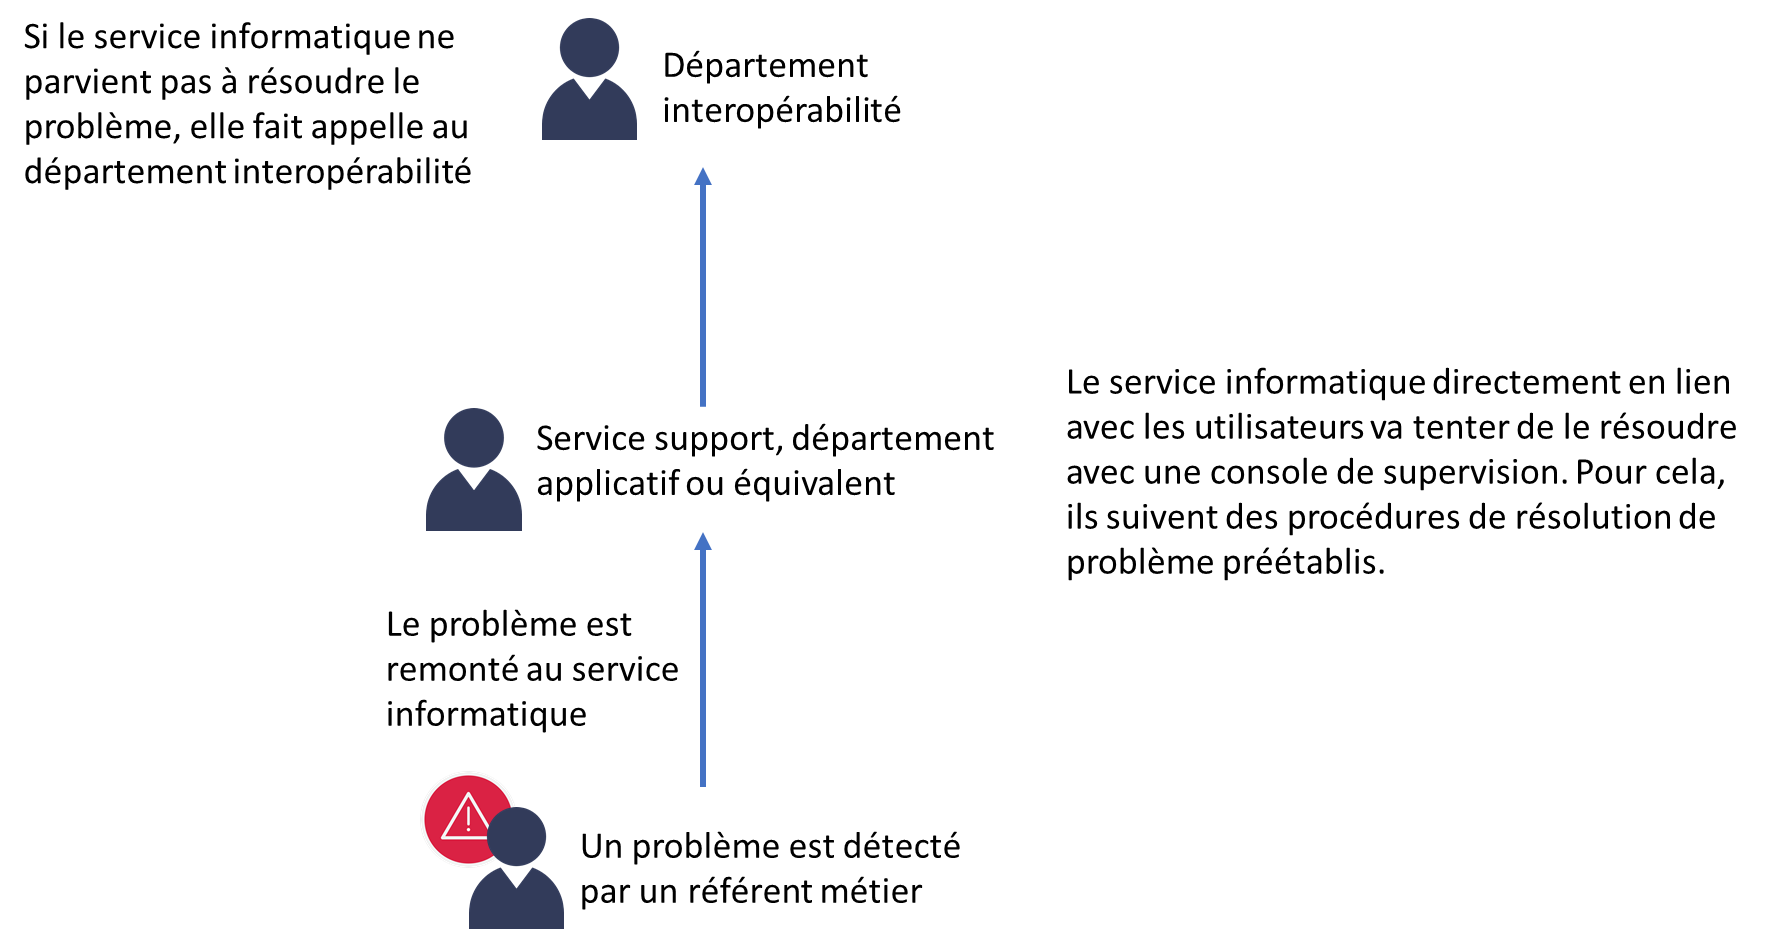
\includegraphics[width=15cm]{../img/user_1.png}
				\caption{\label{resolution_pbs} Processus de résolution d'un problème dans
				Cloverleaf.}
			\end{figure}
			
		\subsubsection{L'enquête permet de dresser une liste des besoins}
			\paragraph{}% Les attentes qui sont ressorties de l'enquête
			Nous remarquons que les avis concernant le rôle des consoles de supervisions
			convergent entre les différentes personnes interrogées. Celles-ci attendent
			de ces outils qu’ils jouent le rôle de tableau de bord clair, simple et si
			possible au design épuré de façon à ce que les informations soient les plus
			lisibles possibles. Une console doit permettre une visualisation rapide des
			erreurs. Elles doivent également permettre leur analyse. La correction des
			erreurs n’est évoquée que comme une fonction secondaire et facultative de
			ces outils.\newline
			D’une manière générale, les utilisateurs son satisfait de l’ergonomie de TC.
			Les principales remarques concernant ce point sont :
			\begin{itemize}
			  \item Le paramétrage des colonnes qui est difficile,
			  \item La lenteur d’affichage des messages,
			  \item Pour certains flux  (les flux externes), il faut parcourir tous les
			  messages pour retrouver ceux ayant un retour négatif.
			\end{itemize}
			Le ressenti global est que les utilisateurs informaticiens, principalement du
			département interopérabilité, ne sont pas spécialement sensibles à
			l’ergonomie des outils de supervision. Ils sont plus soucieux du fonctionnel
			que du design. Mais la plupart des personnes interrogées soutiennent que des
			utilisateurs métiers seraient, quant à eux, plus soucieux du design et de la
			facilité de prise en amin de l’outil. Malheureusement, nous n’avons pu
			interroger de tels utilisateurs.
			
			\paragraph{}% C'est quoi une bonne console
			En résumé, une bonne console est un outil donnant la vision la plus générale
			possible. La console de supervision a pour objectif premier de faire gagner
			du temps à son utilisateur et à permettre une résolution plus rapide des
			problèmes. De ce fait, la console de supervision a pour objectif d’améliorer
			la fiabilité globale de l’EAI, donc du SI.
			
			\paragraph{}% La lise des besoins, classification
			En plus des information que nous avons décrites jusque là, les entetiens nous
			on permi de faire remonter différents besoins des utilisateurs. Ceux-ci l'ont
			été explicitement ou non, et concerne généralement des manques. Voici
			quelques exemples de besoins, la liste complète se trouvant en annexe 3 :
			\begin{itemize}
			  \item Pouvoir trouver facilement la cause des erreurs,
			  \item Voir l'évolution du nombre de messages envoyés par flux au cours du
			  temps,
			  \item Voir la date et heure d'écriture du dernier message,
			  \item Visualiser l'état des flux en temps réel,
			  \item Pouvoir afficher la console sur un écran géan
			\end{itemize}
			Un total de 57 besoins ont été ainsi identifié. Ceux-ci ne sont pas
			spécifiquements lmié à un outil en particulier, ils concernent la supervision
			en général. Certains de ces besoins son d'ailleurs déjà satisfait dans
			TrackCIS, comme c'est par exemple le cas pour : "Pouvoir rejouer les
			messages" ou encore "Avoir un outil utilisable en lecture seule". Ce type de
			besoin nous ayant été remonté par des non utilisateurs de TrackCIS. Nous
			pouvons faire un premier classement des besoins en utilisant les catégories
			suivantes :
			\begin{itemize}
			  \item Besoins concernant les performances,
			  \item Besoins concernant le design, l'ergonomie et la facilité
			  d'utilisation,
			  \item Besoins concernant la résulution des problèmes,
			  \item Besoins concernant les données statistiques,
			  \item Besoins concernant les rôles de la console,
			  \item Les autres besoins
			\end{itemize}
			
			\paragraph{}% Mode de passage des besoins aux fonctionnalités
			Grace à l'enquête terrain, nous en savons un peu plus sur le mode de
			fonctionnement de l'interopérabilité dans le monde hospitalier. Nous en
			savons également d'aventage sur la supervision et les pratiques associée
			ainsi que les paersonnes qui en ont la charge. Enfin, nous avons une liste de
			besoins liés à la supervision des flux. Il est important de préciser que
			nous ne traiterons pas ici tous les besoins de cette liste, mais uniquement
			ceux relatifs à un module statistiques.
			Ce choix est justifié par le fait que :
			\begin{itemize}
			  \item Certain des besoins listés sont déjà satisfait par TrackCIS. En
			  effet, les questions posées lors des entretiens n'étaient pas
			  spécifiquement portées sur cet outil, la plupart des personnes interogées
			  ne l'utilisant pas. Ces besoins ne seront donc pas traités.
			  \item Xperis souhaite apporter toutes les améliorations nécessaires à
			  TrackCIS. Cependant, l'amélioration prioritaire concerne le nouveau module
			  statistique. C'est pourquoi les besoins ayant atrait aux statistiques
			  seront les seuls à être tratiés ici, et donc à être déclinés en
			  fonctionnalités.
			\end{itemize}
			Les élements de cette liste qui ne seront pas traités dans ce mémoire
			pourront servir de base à Xperis pour des amélioration future de l'outil.
			
			\paragraph{}% La lise des besoins, priorisation
			Le classement des besoins permet d'en faciliter la lecture et la
			compréhension, ce qui nous permettra d'imaginer plus aiséement les
			fonctionnalités qui viendrons y répondre. De plus, tous les éléments de cette
			liste ne sont pas égaux, certains besoins compte d'avantage aux yeux des
			personnes interrogée que d'autre. De plus certains ont été cité plus souvant.
			L'enquête que nous avons mené est qualitative et le faible panel de personnes
			interrogées ne nous permet pas de faire des analyse statistiques sur la
			récurence de certains besoins. Cependant, ledit panel est représentatif des
			utilisateurs actuels de TrackCIS, qui ont tous été interrogés. De façon à
			noter l'inportance de chaque besoin pour les utilisateurs, nous proposons de
			nous baser sur le barème présenté dans le tableau \ref{bareme_besoins}
			ainssi que sur le nombre de citation. Le choix des notes dans le barème
			ci-dessous est arbitraire et a pour but de bien différencier les besoins les
			plus prioritaires de ceux qui le sont moins.
			\begin{table}[H]
				\centering
				\begin{tabular}{| p{4cm} | p{8cm} | p{2cm} |}
					\hline
						\thead{Priorité}
						&\thead{Description}
						&\thead{Note}
						\\
					\hline
						Peu important
						&
						S'il est satisfait, ce besoin ne fait qu'améliorer le confort de l'utilisateur. S'il ne l'est pas, rien ne change.
						&
						2
						\\
					\hline
						Important
						&
						S'il est satisfait, améliore l'efficacité de l'utilisateur dans son métier
						&
						3
						\\
					\hline
						Très important
						&
						S'il est satisfait, améliore considérablement l'efficacité de l'utilisateur dans son métier
						&
						5
						\\
					\hline
						Critique
						&
						Besoin qu'il est nécessaire de satisfaire, faute de quoi cela nuira à l'utilisateur.
						&
						8
						\\
					\hline
				\end{tabular}
				\caption{\label{bareme_besoins} Barème choisi pour noter l'importance de
				chaque besoin perçue lors de l'entretien.}
			\end{table}
			Nous calculons la note de chaque besoin avec la formule ci-dessous
			(\ref{besoin_formule}).
			Soit N le nombre de citation et I la note d'importance définie avec le barème du
			tableau \ref{bareme_besoins}.
			\begin{equation}
				\label{besoin_formule}
				Note\ du\ besoin=N\times I
			\end{equation}
			Le résultat de cette priorisation se trouve dans la colonne "Note besoin" du
			tableau de l'annexe 3.
	
	\subsection{La liste des besoins permet de dresser une liste de fonctionnalités}
		\paragraph{}% On ne se concentre que sur les besoins liés aux stats
		Nous avons dressé et analysé une liste de besoins émanant d'utilisateur
		concernant la supervision. L'objectif est maintenant, à partir de cette liste,
		de dresser une liste de fonctionnalités.
		
		\subsubsection{De la liste des besoins à la liste des fonctionnalités}
			\paragraph{}% C'est quoi une fonctionnalité ??
			Une fonctionnalité est un service rendu par une application à un utilisateur.
			Par exemple, la version actuelle de TrackCIS permet à l'utilisateurs de
			consulter la liste des messages qui sont passé dans un flux. Ceci est une
			fonctionnalité et elle répond à un besoin de l'utilisateur. En l'occurence le
			besoin en question pourrait être "consulter la liste des messages transitant
			par le fux". Dans ce cas-ci, le passage du besoin à la fonctionnalité est
			évidente, puisque ls deux sont formulable de la même manière. Mais dans ce
			cas quelle est la différences entre les deux ? Un besoin n'est pas lié à un
			outil en particulier, c'est une volonté de l'utilisateur lié à un manque. Une
			fonctionnalité est elle liée à un outil particulier, puisqu'il s'agit d'un
			service rendu par cet outil.
		
			\paragraph{}% La liste des fonctionalités
			On peut établir des fonctionnalités à partir des besoins que l'on a retenu.
			Une fonctionnalité est une réponse à un besoin. Cette réponse est portée par
			un outil, en l'occurence TrackCIS. Les besoins retenus sont aux nombre de 33.
			Nous imaginons à partir de là une liste composée de 30 fonctionnalités
			(annexe 4) regroupées en 8 grands ensembles :
			\begin{itemize}
			  \item Visualisation du niveau de disponibilité du flux.
			  \item Visualisation de la date et heure du dernier message passé.
			  \item Visualisation de l’historique des messages.
			  \item Visualisation des ressources serveur.
			  \item Administration des statistiques.
			  \item Exporter les données statistiques.
			  \item Facilitation de l’utilisation.
			\end{itemize}
			
		\subsubsection{Priorisation des fonctionnalités liées aux statistiques}
			\paragraph{}% But de la priorisation des fonctionnalités
			De la même manière que nous avons priorisé les besoin, nous cherchons ici à
			prioriser les fonctionnalités qui en découlent. L'objectif de cela est
			d'anticiper le développement des fonctionnalités : les plus importantes
			devant être implémentées en premier. Il nous faut donc mettre en place un
			barème permettant d'ordonner les fonctionnalités les unes par rapport aux
			autres. Nous allons nous ader pour cela du diagramme FODA (Feature Oriented
			Domain Analysis).
			
			\paragraph{}% Présentation FODA
			Le diagramme FODA est une représentation graphique des différentes
			fonctionnalités de l’application (Kang, 1990). Il est organisé en features.
			Une feature est une macro fonctionnalité. A l’intérieur de chaque feature
			peuvent se trouver d’autres fonctionnalités, plus précises, sous lesquelles
			peuvent s’en trouver d’autres, etc. Les feuilles de l’arbre ainsi formé
			(correspondant au niveau de fonctionnalité le plus détaillé) correspondent à
			des parties fonctionnelles de l’application qui seront développées.\newline
			La figure \ref{foda_legende} présente le principe de base du diagramme FODA.
			La \textit{feature} 1 est obligatoire (point noir), elle correspond à la
			fonctionnalité d'un produit minimum viable (PMV). La \textit{feature 2} est
			facultative (point blanc), elle correspond à une fonctionnalité qui pourra être
			développée dans des versions plus évoluées ou plus personnalisées de
			l’outil. Elle n’est pas indispensable au fonctionnement ni à la mise sur le
			marché, mais rend tout de même un service intéressant pour l'utilisateur.
			\begin{figure}[H]% Légende du FODA
				\centering
				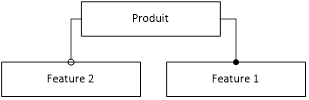
\includegraphics[width=7cm]{../img/foda_legende.png}
				\caption{\label{foda_legende} Principe du diagramme FODA.}
			\end{figure}
			
			\paragraph{}% FODA de TrackCIS stats
			Nous mettons en pratique cette classification en concertation avec l'équipe
			d'Xperis. Cette séparation entre fonctionnalité optionnelles ou faisant parti
			du PMV refète donc le choix de l'entreprise. Pour tenir également compte des
			priorités des utilisateurs interrogés durant l'enquête, nous proposons la
			formule ci-dessous. Soit Bi la note d'un besoin donnée,
			\begin{math}\sum Bi\end{math} représente la somme des notes des besoins qui
			sont satisfaits par cette fonctionnalité. On a la formule \ref{fonctio_nopmv}
			pour une fonctionnalité notée comme facultative et la formule
			\ref{fonctio_pmv} pour une fonctionnalité notée comme obligatoire. Les notes
			obtenues pour chaque fonctionnalités sont présentées dans la colonne "Note
			de fonctionnalité" du tableau de l'annexe 4.
			\begin{equation}
				\label{fonctio_nopmv}
				Note\ de\ la\ fonctionnalite=\sum Bi
			\end{equation}
			\begin{equation}
				\label{fonctio_pmv}
				Note\ de\ la\ fonctionnalite=2\times \sum Bi
			\end{equation}
			
		\subsubsection{Le nouveau module se découpe en huits grands groupes de
		fonctionnalités}
			\paragraph{}
			Les figures \ref{foda_1} et \ref{foda_2} représentent l'ensemble des
			fonctionnalités du module statistique de TrackCIS sous forme de diagramme
			FODA . Chaque feature correspond à un des 8 grands
			ensembles de fonctionnalité décrit précédemment. Attardons nous sur chaque
			feature. 
			\begin{figure}% foda 1
				\centering
				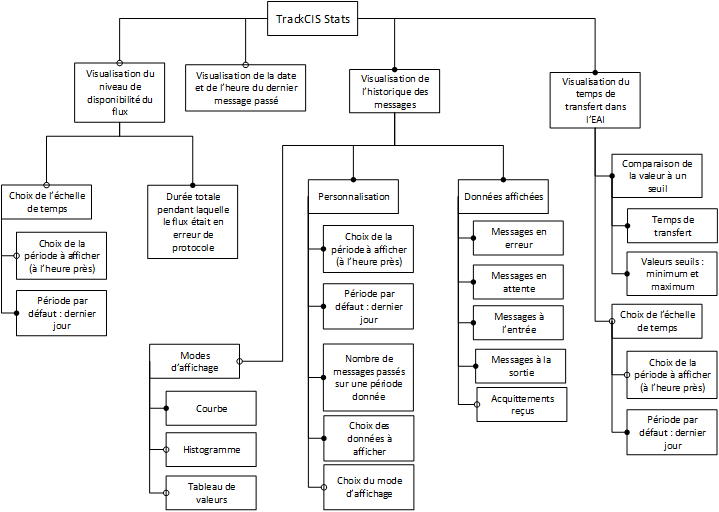
\includegraphics[width=17cm]{../img/part2/foda_1.png}
				\caption{\label{foda_1} Diagramme FODA pour le module statistique de
				TrackCIS (première partie).}
			\end{figure}
			\begin{figure}% foda 2
				\centering
				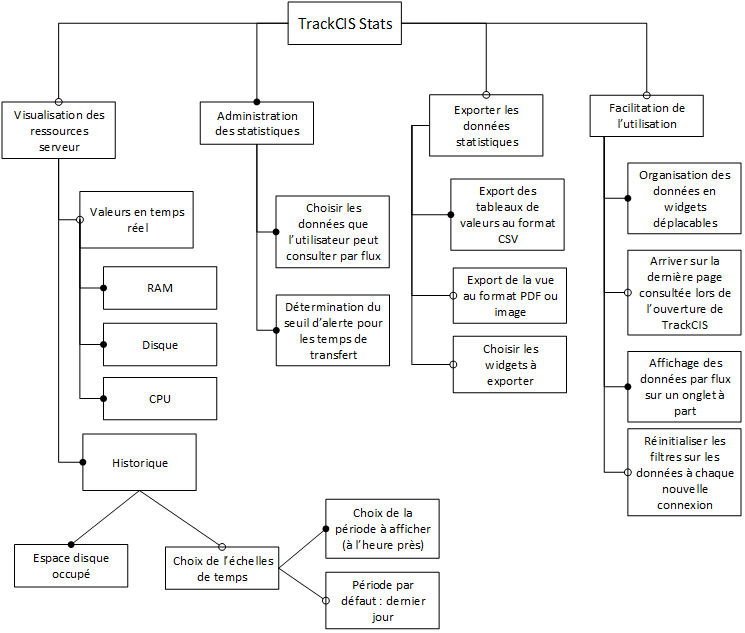
\includegraphics[width=17cm]{../img/part2/foda_2.png}
				\caption{\label{foda_2} Diagramme FODA pour le module statistique de
				TrackCIS (deuxième partie).}
			\end{figure}
			
			\paragraph{Visualisation du niveau de disponibilité du flux.}
			
			
			\paragraph{Visualisation de la date et heure du dernier message passé.}
			
			\paragraph{Visualisation de l’historique des messages.}
			
			\paragraph{Visualisation des ressources serveur.}
			
			\paragraph{Administration des statistiques.}
			
			\paragraph{Exporter les données statistiques.}
			
			\paragraph{Facilitation de l’utilisation.}
			
	
	\subsection{Des fonctionnalités vers les cas d'utilisation}
		\paragraph{}
		Nous savons maintenant quelles sont les services que doit rendre notre nouveau
		module.
		
		\subsubsection{État de l'art sur les consoles de supervision et la visualisation de données}
			\paragraph{}
			Pour cet état de l’art nous nous baserons sur des outils remplissant des
			fonctions similaires à celles que l’on attendrait de TrackCIS. Cet état de
			l’art est réalisé dans le but du développement du module statistique. Nous
			nous attarderons donc, dans l’analyse des exemples, sur :
			\begin{itemize}
			  \item Les données qui sont affichée et leurs rôles,
			  \item La manière dont ces données sont représentées (courbe, histogramme,
			  jauge...), pourquoi elles sont représentées de la sorte et si cela semble
			  efficace et ergonomique du point de vue de l’utilisateur.
			\end{itemize}
			Nous analyserons ici 2 outils : TradeXpress et M12.
			
			\paragraph{TradeXpress :}
			TradeXpress est une plateforme d’intégration B2B. L’outil permet de connecter
			les application d’une entreprise à celles de ses partenaires (clients,
			fournisseurs…). TradeXpress n’est pas spécialisé dans un domaine en
			particulier. Il permet de gérer l’intégralité des flux, il va bien au-delà
			de la simple supervision. Cependant, certaines de ces fonctionnalités sont
			axés supervision, ce sont celles qui nous intéressent ici. La figure
			\ref{trade_xpress} présente la page de monitoring des flux de la console.\newline
			La vue se divise en deux parties aux rôles différents : une partie consacrée
			à l’état du système, une autre dédiée à la supervision. La première partie
			montre une vision de l’état actuel (en temps réel) du serveur. La partie
			supervision offre deux vision :
			\begin{itemize}
			  \item Une au jour à l’aide de jauges montrant le nombre de messages ou
			  documents transitant par l’EAI. On peut voir juste en dessous de l’encadré
			  gris un bouton permettant de sélectionner la date.
			  \item Un historique à la semaine du volume de messages passés pour chaque
			  domaine. L’utilisateur peut choisir les données ainsi que la semaine à
			  afficher.
			\end{itemize}
			Le design de l’outil est simple et relativement classique. Les informations
			utiles à l’utilisateur occupent un maximum de place sur la page. Il y a le
			moins de superflu possible : pas de cadre autour des parties et seulement
			cinq couleurs différentes.\newline
			Pour la partie supervision, l’utilisateur ne peut pas sélectionner la
			période de temps, il doit se contenter de visualiser les données d’un jour
			ou d’une semaine particulière. Ceci restreint les possibilités de
			visualisation, mais simplifie l’utilisation de la console.\newline
			Pour que les jauges soient pertinentes il faut qu’elles soient calibrées avec
			une valeur minimum et maximum. La documentation disponible en ligne ne précise
			pas s’il est possible de calibrer ces jauges, ni à qui revient ce rôle.
			\begin{figure}[h]
				\centering
				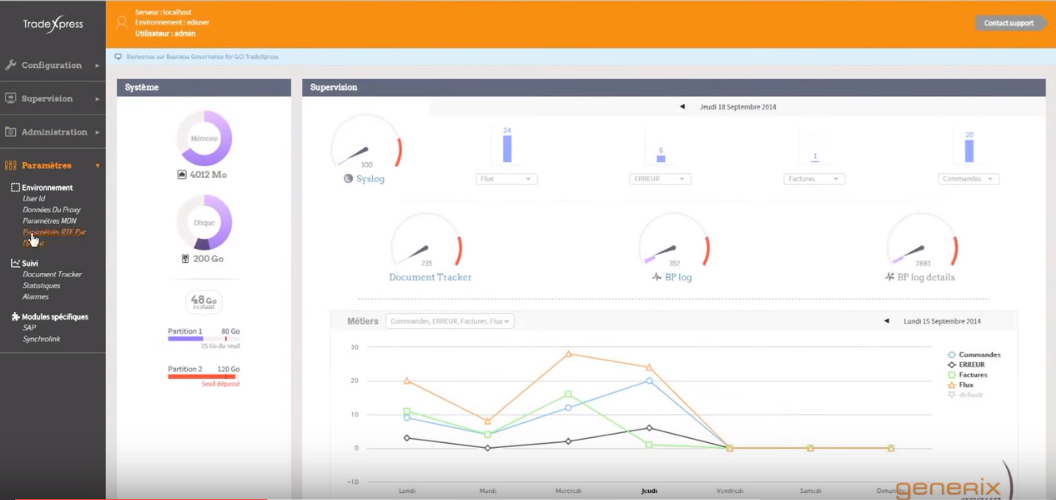
\includegraphics[width=17cm]{../img/part2/trade_xpress.png}
				\caption{\label{trade_xpress} Tableau de bord de l'outil Trade Xpress.}
			\end{figure}
			
			\paragraph{M12 :}
			M12 est une console permettant de monitorer des flux existant, principalement
			les flux basés sur des web services. La console permet de générer des
			alertes (par exemple des alertes mail) en cas de problème, et de rejouer les
			flux.
			\begin{figure}[h]
				\centering
				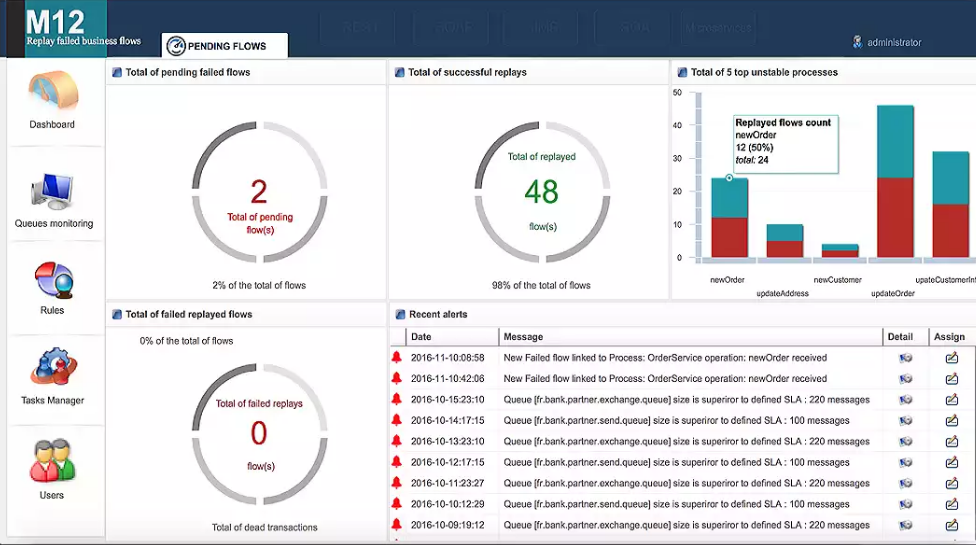
\includegraphics[width=17cm]{../img/part2/m12.png}
				\caption{\label{m12} Tableau de bord de l'outil M12.}
			\end{figure}
			
		\subsubsection{Choix des modes de visualisation par le biais de maquettes}
			\paragraph{}
			Texte de la sous sous partie
		\subsubsection{Création de scénarios d'utilisation}
			\paragraph{}
			Texte de la sous sous partie

	\section{Phase de développement : implémentation d'un module statistique}
	\paragraph{}
	Intorduction de la partie.
	
	\subsection{Une gestion de projet en mode agile}
		\paragraph{}
		Introduction de la sous partie.
		 
		\subsubsection{Les grands principes de l'agilité}
		\subsubsection{Élaboration du backlog}
	
	\subsection{TrackCIS, une application web en deux parties}
		\paragraph{} 
		Introduction de la sous partie.
		 
		\subsubsection{Qu'est-ce qu'une application web ?}
		\subsubsection{TrackCIS est composé d'un frontal et d'une API}
		\subsubsection{Le frontal est développé en java J2EE}
		\subsubsection{L'API permet de communiquer avec Cloverleaf}
	
	\subsection{L'analyse technique permet l'implémentation du nouveau module à l'existant}
		\paragraph{}
		Introduction de la sous partie.
		
		\subsubsection{Structure des données disponibles dans l'EAI}
		\subsubsection{Nouvelle architecture de l'application}
		\subsubsection{Choix de la bibliothèque graphique}
	
	\subsection{Bilan de la phase de développement et suite du projet}
		\paragraph{}
		Introduction de la sous partie.
		
		\subsubsection{Les fonctionnalités implémentées}
		\subsubsection{Suites possibles du projet pour Xperis}
	
	\section*{Conclusion}
		\paragraph{}
		Paragraphe de conclusion.

  \newpage
  \bibliography{../biblio/biblio}
	\backmatter
	
	

	\nocite{*}
	
	
	%\appendix
	\begin{appendix}
		\tocless\chapter{Questionnaire d'enquête dans sa dernière version}
	\paragraph{Identification de la personne, exploration du contexte}
	\begin{itemize}
	  \item 1.1. Quel est votre métier ? Quels sont vos rôles et responsabilités ?
	  \item 1.2. *Comment est structuré le service informatique dans votre
	  établissement ? Quels sont les différentes fonctions que l’on y retrouve ? Combien de personnes ?
	  \item 1.3. *Quels sont vos liens avec les autres services / les autres
	  fonctions ? (Coopération, liens hiérarchiques, conflits, …)
	\end{itemize}
	
	\paragraph{Utilisation et utilisateurs de cloverleaf et problématiques liés à la
	supervision des flux}
	\begin{itemize}
	  \item 2.1. *Etes-vous amenés à utiliser l’EAI Cloverleaf :
	  	\begin{itemize}
	  	  \item Par le biais de l’IDE ? Si oui, pour quoi ?
	  	  \item Par le biais d’une console de supervision ? Si oui, laquelle et pour
	  	  quoi ?
	  	\end{itemize}
	   \item 2.2. Quelle part de votre temps allouez-vous à l’utilisation de
	   Cloverleaf ? (IDE et consoles de supervision) Estimez-vous que ce soit trop ? Pas assez ?
	   \item 2.3. Comment évalueriez-vous votre niveau de maîtrise de :
	   	\begin{itemize}
	  	  \item L’IDE de Cloverleaf ? Pourquoi ?
	  	  \item La/les consoles de supervision ? Pourquoi ?
	  	\end{itemize}
	   \item 2.4. *Quelles sont les autres personnes qui, dans votre établissement,
	   sont amenées à utiliser Cloverleaf par le biais :
	   	\begin{itemize}
	  	  \item De l’IDE ? Pour quoi ?
	  	  \item De la/les consoles de supervision ? Pour quoi ?
	  	\end{itemize}
	\end{itemize}
	
	\paragraph{Attentes par rapport aux consoles de supervision}
	Question généraliste (ne s’applique pas à un outil en particulier) :
	\begin{itemize}
	  \item 3.1. *Selon vous, quels sont les 3 principaux rôles qu’une console de
	  supervision d’un EAI tel que Cloverleaf ? Autrement dit, quels sont les 3
	  principales problématiques auxquelles de telles plateformes répondent ?
	\end{itemize}
	
	\paragraph{Questions portant sur les consoles actuelles}
	Consoles de supervisions utilisées :
	\begin{itemize}
	  \item (1) TrackCIS
	  \item (2) Glaobal Monitor
	  \item (3) EAI Supervision
	  \item (4) Autres, préciser
	\end{itemize}
	Pour chaque outil utilisé :
	\begin{itemize}
	  \item 4.1. *Trouvez-vous que l’utilisation de cet outil est simple ? Pourquoi
	  ? Quelles sont les difficultés que vous rencontrez (ergonomie, prise en main…) ?
	  \item 4.2. *Selon vous, quelle est le plus gros atout de cet outil ?
	  \item 4.3. Quelles sont les fonctionnalités que vous êtes amenés à utiliser le
	  plus souvent sur cet outil ? Pour quoi ?
	  \item 4.4. *Selon vous, quelle est la plus grosse faiblesse de l’outil ?
	  \item 4.5. *Citez au moins 3 fonctionnalités qui vous semble manquer dans cet
	  outil ?
	  \item 4.6. *Si l’outil pouvait afficher des statistiques sur les flux (comme
	  par exemple le nombre de messages en erreur heure par heure, …), quelles
	  données seraient les plus pertinentes d’afficher selon vous ? (En proposer au
	  moins 3 en précisant le mode d’affichage (graphique, histogramme, tableau,
	  …))
	  \item 4.6 bis. *Quelles données statistiques (présentent dans le status dans
	  l’IDE) vous sont les plus utiles au quotidien ?
	  \item 4.7. Que pourrait vous apporter de telles statistiques ? (Plus
	  d’efficacité dans la gestion des messages, meilleur vision globale…) En quoi
	  cela changerait vos pratiques ?
	\end{itemize}
	
	paragraph{Autres questions}
	\begin{itemize}
	  \item 5.1. Dans votre établissement, qui prend la décision d’achat des
	  solutions telles que Cloverleaf ou les consoles de supervision ?
	  \item 5.2. Pour quelles raisons (si vous les connaissez) votre établissement a
	  choisi d’adopter la/les consoles de supervision ?
	  \item 5.3. *Nous sommes arrivés au bout de ce questionnaire. Avez-vous autre
	  chose à ajouter ?
	\end{itemize}
	
	*Questions les plus importantes.
		\tocless\chapter{Comptes rendu d'entretiens}
\paragraph{Identification de la personne, exploration du contexte}
	\begin{itemize}
	  \item 1.1. Quel est votre métier ? Quels sont vos rôles et responsabilités ?
	  \begin{description}
	  	\item[Toulouse~:] Responsable intégration / urbanisation. L’objectif du pôle
	  	intégration est d’étudier tous les besoins liés à l’interopérabilité. Ils
	  	sont sollicités dès qu’un chef de projet demande la mise en place d’un
	  	flux, dès qu’une nouvelle application arrive.
	  	\item[Tours~:] Fait partie de l’équipe intégration. Equipe de 2 personnes.
	  	En charge de tous les flux, principalement les flux médicaux. S’occupe un
	  	peu moins des flux administratifs (flux de la logistiques…). Donc
	  	principalement des flux concernant les patients.\\
		L’établissement dispose de plusieurs EAI.
	  	\item[Rouen~:] Fait partie de l’équipe intégration et flux (département RIF),
	  	en binôme avec une collègue, il s’occupe des différents EAI, dont Cloverleaf.
	  	\item[Brest~:] Personnes présentes : 3 personnes utilisant Cloverleaf par le
	  	biais de l’IDE et de EAI Supervision. Profils plutôt techniques.
	  	\item[Metz~:] Travail dans le secteur exploitation, s’occupe principalement
	  	de la gestion des flux.
	  \end{description}
	  
	  \item 1.2. Comment est structuré le service informatique dans votre
	  établissement ? Quels sont les différentes fonctions que l’on y retrouve ? Combien de personnes ?
	  \begin{description}
	  	\item[Toulouse~:] L’interopérabilité : Echanger des données entre
	  	applications métier. Ces applications sont réparties en domaines : Soin,
	  	Médicotechnique, Logistique, Administratif\\
		Il y a différents niveaux liés à l’interopérabilité : L’urbanisation,
		architecture globale du SI, Normes des données et mise en œuvre de ces normes,
		Intégration de nouvelles applications -	Surveillance des flux (supervision)
		Bientôt un pôle exploitation va être créé. Ce pôle s’occupera de la
		supervision des flux.
	  	\item[Tours~:] 3 départements : \\
		-	Administratif : admission patient, logistique, finances, etc.\\
		-	Médicale : Applications médicales\\
		-	Technique : réseau, matériel…
	  	\item[Rouen~:]
	  	\begin{figure}[H]
			\centering
			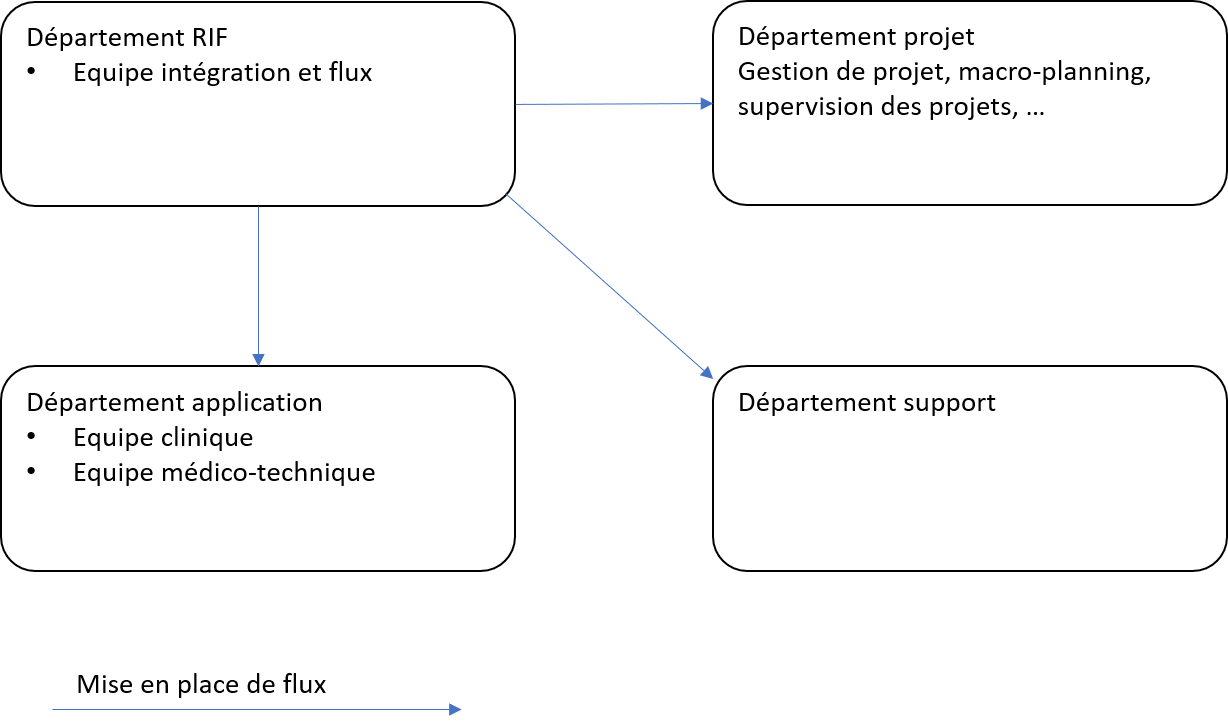
\includegraphics[width=15cm]{../img/annexes/orga_rouen.png}
		\end{figure}
		Le département application est le plus gros demandeur de flux. Les
		départements application et support ont des équipes d’informaticiens qui
		n’ont pas forcément des compétences sur Cloverleaf.
	  	\item[Metz~:]
	  	\begin{figure}[H]
			\centering
			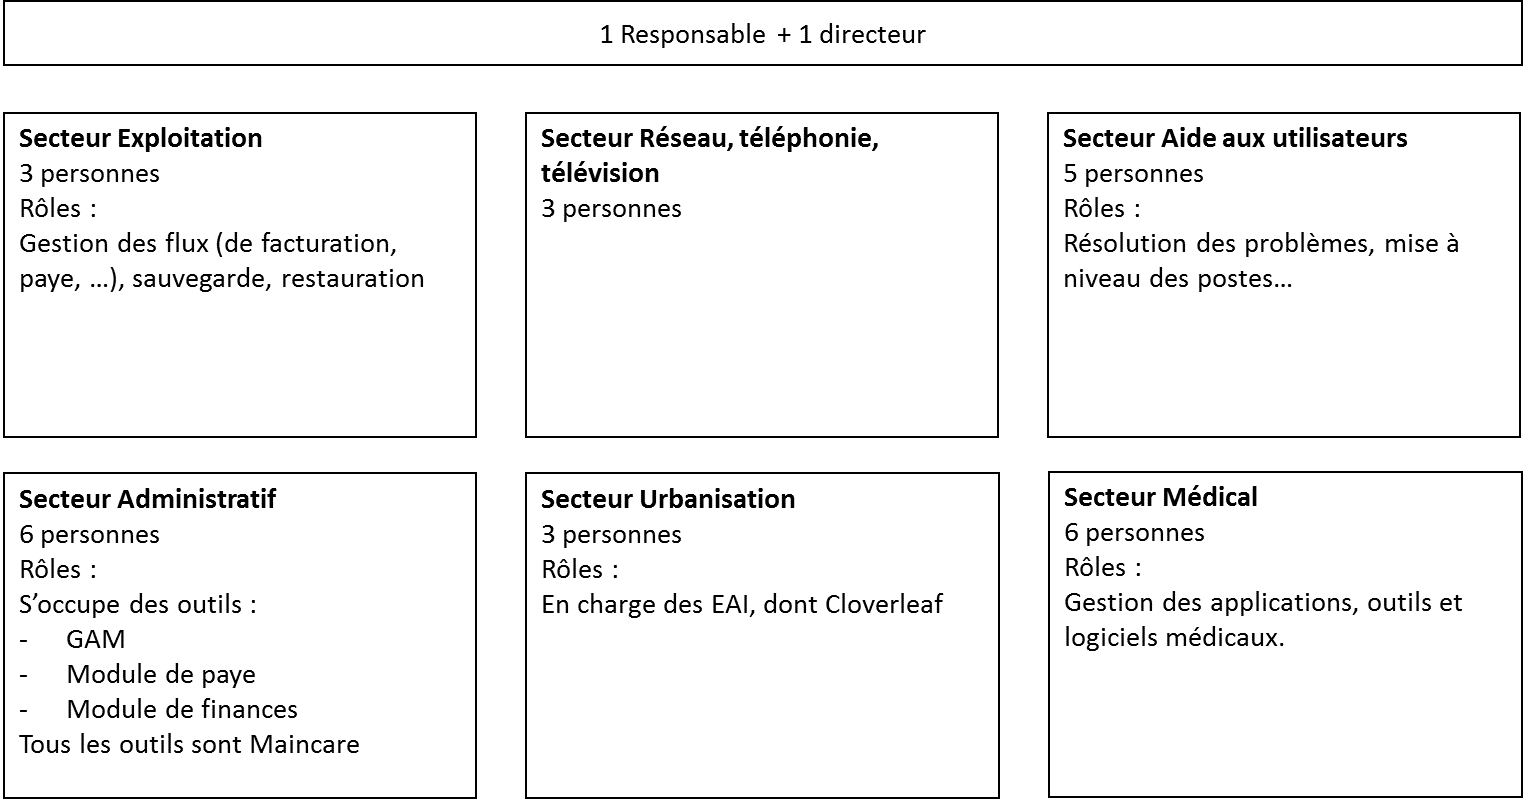
\includegraphics[width=15cm]{../img/annexes/orga_metz.png}
		\end{figure}
	  \end{description}
	  
	  \item 1.3. Quels sont vos liens avec les autres services / les autres
	  fonctions ? (Coopération, liens hiérarchiques, conflits, …)
	  \begin{description}
	  	\item[Tours~:] L’équipe intégration se rattache officiellement au
	  	département médical, mais travail autant avec le département administratif
	  	que médical.
	  	\item[Metz~:] En lien principalement avec le secteur administratif. Peu de
	  	liens avec le secteur réseau, téléphonie, télévision, le secteur médical et
	  	le secteur aide aux utilisateurs. Le secteur médical supervise ses propres
	  	flux (flux issus des applications médicales. Le secteur exploitation
	  	s’occupe essentiellement des flux administratifs. Ne s’occupe pas de
	  	Cloverleaf, c’est le secteur urbanisation qui a la charge du bon
	  	fonctionnement de l’EAI. Le secteur exploitation s’occupe de superviser les
	  	flux.
	  \end{description}
	\end{itemize}
	
	\paragraph{Utilisation et utilisateurs de cloverleaf et problématiques liés à la
	supervision des flux}
	\begin{itemize}
	  \item 2.1. Etes-vous amenés à utiliser l’EAI Cloverleaf :
  	  \begin{description}
	  	\item[Toulouse~:] Démarrage de Cloverleaf en 2006 avec le MIPIH. A l’époque,
	  	le rôle du pôle intégration était seulement de faire de la supervision, le
	  	MIPIH s’occupait de tout. Puis le choix a été fait de monter en compétence
	  	sur l’EAI, notamment sur le développement de flux. L’objectif était de
	  	devenir autonome sur le développement de flux, ce qui est le cas
	  	aujourd’hui. Utilisation des consoles de supervision :\\
	  	Global Monitor :\\
	  	Utilisé pour le niveau 1 (surveillance des flux). Utilisé aussi par les
	  	personnes d’astreintes pour surveiller leurs propres flux. Les personnes
	  	d’astreintes ont des restrictions sur la console.
		Global Monitor est utilisé par les techniciens et ingés de la DSIO et par le service
		intégration.\\
	  	TrackCIS :\\
	  	L’objectif est de le mettre à disposition des référents techniques.
		Les référents techniques sont des personnes métier qui sont les interlocuteurs
		privilégiés avec la DSIO. Ces personnes (pharmaciens, infirmières, médecins…)
		remontent les problèmes quand ils surviennent à la DSIO. Quand il s’agit d’un
		problème d’interopérabilité (par exemple un message qui ne transite pas
		correctement d’une application à une autre), la DSIO fait appel au service
		intégration pour le résoudre (si elle n’y arrive pas elle-même).\\
	  	Cette procédure de résolution fait appel à beaucoup d’intermédiaires et
	  	prend beaucoup de temps. L’objectif de TC est de simplifier la majorité des
	  	cas de problème en donnant au référent métier un outil (TrackCIS) leur permettant
	  	de résoudre eux-mêmes certains problème (en rejouant ou en modifiant les
	  	messages).\\
		De plus, la supervision des flux est une perte de temps pour le pôle
		intégration.\\
		Utilisation des alertes Cloverleaf par le pôle intégration et par les équipes
		DSIO.
	  	\item[Tours~:] Principalement par le biais de l’IDE, un peut avec GM.\\
		TrackCIS n’est pas encore utilisé en production, l’outil n’est pas encore
		paramétré.
	  	\item[Rouen~:] Affichage de GM sur un écran géant. Visualisation de l’état
	  	des flux, des messages en erreur en temps réel. Cet écran affiche aussi 2
	  	autres consoles de supervision pour leurs autres EAI.\\
		L’IDE est installée sur les postes. Utilisé plus pour le paramétrage des flux,
		le diagnostic et la correction des erreurs.\\
		TrackCIS (TC) n’est pas utilisé. Il est en cours de paramétrage. Ils
		réfléchissent encore sur le meilleur moyen de l’utiliser.\\
		Font peu de transformation.
	  	\item[Brest~:] Utilisation de Cloverleaf via l’IDE et EAI Supervision.
	  	\item[Metz~:] N’utilise que TrackCIS pour gérer les flux Cloverleaf.
	  \end{description}
	  
	   \item 2.2. Quelle part de votre temps allouez-vous à l’utilisation de
	   Cloverleaf ? (IDE et consoles de supervision) Estimez-vous que ce soit trop ? Pas assez ?
	   \begin{description}
	  	\item[Metz~:] En moyenne 1,5h par jour et par personne. N’estime pas que
	  	c’est une perte de temps.
	  \end{description}
	  
	   \item 2.3. Comment évalueriez-vous votre niveau de maîtrise de :
	   \begin{description}
	  	\item[Toulouse~:] L’équipe intégration a pour but d’être autonome sur la
	  	création de flux.
	  	\item[Rouen~:] Bonne maîtrise
	  	\item[Brest~:] Une bonne autonomie par rapport à Cloverleaf, bon niveau de
	  	maitrise :\\
		-	L’établissement a mené des négociations avec Maincare dans le but de
		devenir plus autonome vis-à-vis de Cloverleaf •	De ces négociations ont
		découlées des formations de Maincare, notamment sur la création de flux et de
		threads.\\
		-	Le CHU est autonome pour la création de nouveaux flux. Cependant, Maincare
		doit valider chaque nouveau flux mis en place.\\
		-	L’équipe maîtrise la transformation de messages (procédures TCL).\\
		L’équipe SI est très curieuse sur le fonctionnement de l’EAI et très
		désireuse de monter en compétence. Pour eux Cloverleaf n’est pas simplement
		une « boite noir » gérée uniquement par Maincare.
	  	\item[Metz~:] Faible niveau de maitrise de l’EAI, ne maîtrise que la
	  	supervision de certains flux via TrackCIS.
	  \end{description}
	  
	   \item 2.4. Quelles sont les autres personnes qui, dans votre établissement,
	   sont amenées à utiliser Cloverleaf par le biais :
	   	\begin{description}
		  	\item[Toulouse~:] Cloverleaf est trop complexe pour des utilisateurs
		  	métiers. D’où l’intérêt d’une console telle que TC. Ça leur permettrait de
		  	vérifier si tel message est bien passé.\\
			Rq : Plus de 30 000 messages passent quotidiennement sur les flux
			identité-mouvement.\\
			A l’heure actuelle, aucun référent métier n’utilise encore TC, même si des
			tests ont déjà été effectués avec ce genre d’utilisateur. Aujourd’hui TC est
			utilisé par les équipe de la DSIO pour réaliser des tests lors de la mise en
			place de flux au moment de la recette fonctionnelle.
		  	\item[Tours~:] GM est utilisé par les personnes d’astreintes. Ce sont des
		  	personnes utilisatrices d’application, pas forcément des informaticiens.
		  	Ils n’ont qu’un accès restreint aux flux qui les intéresse.\\
			Ne destine pas TrackCIS à des utilisateurs métier. Crain que ça soit trop
			compliqué pour eux de gérer les flux, risques d’erreurs de leurs parts
			surtout dans la correction des erreurs. Ou alors juste en lecture seul (sans
			possibilité de rejouer les messages). « On ne peut pas déléguer la fonction
			de rejoue à tout le monde ».\\
			L’outil est d’avantage destiné à des informaticiens, ayant une connaissance
			minimum de l’IDE. Ces mêmes informaticiens veulent en effet savoir ce qu’il
			s’est passé en cas de problème.
		  	\item[Rouen~:] Concernant TrackCIS :\\
			Pas d’utilisateurs actuels. Il est prévu que ce soit des personnes métier
			(EAC) qui utilisent TC, donc pas des informaticiens (des référents
			informatiques). Par exemples le personnel chargé de l’accueil des patients
			pour bien vérifier que les données qu’ils saisissent diffusent bien dans les
			autres services. Rq : pas de cas d’utilisations très claires pour l’instant
			au niveau de ce type d’utilisateur.\\
			L’utilisation de TC est ici restreinte au domaine concerné par l’utilisateur
			métier.\\
			Concernant Global Monitor :\\
			Tout informaticien travaillant de près ou de loin sur des flux : les
			informaticiens du département application, du département support et bien
			sur l’équipe intégration et flux.\\
			L’utilisation de GM est ici également restreinte au domaine concerné par
			l’utilisateur.\\
			EAI supervision :\\
			Utilisé par les informaticiens du département application (et aussi un peu
			support) pour gérer les flux Maincare et l’intégration des messages dans les
			applications de l’éditeur. C’est le département support qui fait le lien
			avec Maincare en cas de problème.
		  	\item[Brest~:] Les mêmes personnes utilisent Cloverleaf via son IDE et EAI
		  	Supervision. Ces personnes sont très compétentes sur l’EAI. La console de
		  	supervision est utilisée pour gagner du temp et visualiser rapidement les
		  	messages en erreur, faire des modifications sur les messages et rejouer.
		  	\item[Metz~:] Il a essayé de donner le suivi des flux aux utilisateurs des
		  	applications administratives, mais sans succès. Aucun utilisateur ne
		  	semble vouloir s’occuper de ça, estimant ne pas avoir le temps et que ça
		  	n’est pas leur rôle de le faire. De plus, une pratique est déjà bien
		  	installée : si un envoi de message ne fonctionne pas, l’utilisateur appel
		  	d’office le service exploitation.\\
			C’est le seul utilisateur de TrackCIS dans l’établissement.
		  \end{description}
	\end{itemize}
	
	\paragraph{Attentes par rapport aux consoles de supervision}
	Question généraliste (ne s’applique pas à un outil en particulier) :
	\begin{itemize}
	  \item 3.1. Selon vous, quels sont les 3 principaux rôles qu’une console de
	  supervision d’un EAI tel que Cloverleaf ? Autrement dit, quels sont les 3
	  principales problématiques auxquelles de telles plateformes répondent ?
	  \begin{description}
	  	\item[Toulouse~:] Pouvoir visualiser très rapidement les problèmes ; Avoir
	  	une ergonomie simple ; Pouvoir agir pour dépanner (mais ça c’est
	  	facultatif).\\
	  	Le rôle premier d’une console de supervision est de pouvoir
	  	rapidement diagnostiquer un problème. La résolution du problème est un
	  	fonction « bonus » de la console.
	  	\item[Tours~:] Vision immédiate (de l’état d’un flux, des messages) et sans
	  	besoin de scroller.\\
		En cas d’anomalie, permet d’analyser le problème.
	  	\item[Rouen~:] Varie en fonction du type d’utilisateur de la console.
	  	\item[Brest~:] Utilisation possible par les personnes en astreintes en
	  	lecture seul (ce n’est pas le cas à Brest)
	  	\item[Metz~:] <<~Avoir une vue bien claire avec un message allé et un
	  	message retour. Visualiser les erreurs avec leur contenu et leur
	  	origine.~>>\\
	  	Un affichage épuré, simple, pas surchargé en informations.
	  \end{description}
	\end{itemize}
	
	\paragraph{Questions portant sur les consoles actuelles}
	Pour chaque outil utilisé :
	\begin{itemize}
	  \item 4.1. Trouvez-vous que l’utilisation de cet outil est simple ? Pourquoi
	  ? Quelles sont les difficultés que vous rencontrez (ergonomie, prise en main…) ?
	  \begin{description}
	  	\item[Toulouse~:] TrackCIS est parfaitement adapté aux référents métiers.
	  	Très simple à utiliser, pas besoin de doc.
	  	\item[Tours~:] TrackCIS : pas encore utilisé en production.\\
		Global Monitor : pas de retours négatifs des utilisateurs concernant
		l’ergonomie, la facilité d’utilisation. Mais GM est lent, l’outil se bloque
		parfois. Au niveau de l’ergonomie, l’espace de la page / des widget est parfois
		très mal occupé sur certains écrans (éléments dans un coin ou tout en bas et
		rien autour).
	  	\item[Rouen~:] TrackCIS : simple, épuré et ergonomique\\
		Global Monitor : peu ergonomique (surtout pour la rejoue de messages), plus
		difficile à prendre en main
	  	\item[Brest~:] (Pour EAI Supervision) Outil simple à utilisés, relativement
	  	intuitif, mais la prise en main est difficile. Une vue tableau de bord pratique.
	  	\item[Metz~:] Remarque : il utilise conjointement 2 versions de TrackCIS :
	  	la 1.2.0 pour les flux GAM et GEF (flux internes) et la 1.2.93 pour les
	  	flux externes.\\
	  	Il trouve difficile de jongler entre les 2 TrackCIS, aimerait un affichage
	  	unique pour gérer les flux internes et les flux externes.\\
		Il souhaiterait arriver sur la liste des flux du jour en arrivant sur la page
		d’accueil de TrackCIS (bouton <<~flux du jour~>> ?). Actuellement, il arrive
		sur les flux correspondant à son dernier filtre. Il est obligé de refiltrer les
		flux à la date d’aujourd’hui chaque jour. Car le suivi des flux <<~se fait au
		jour le jour~>>.
	  \end{description}
	  
	  \item 4.2. Selon vous, quelle est le plus gros atout de cet outil ?
	  \begin{description}
	  	\item[Toulouse~:] TrackCIS permet de donner de l’autonomie aux personnes dont
	  	l’EAI n’est pas le métier. « Les gens sont très contents d’avoir une
	  	certaine autonomie. » TrackCIS permet de renommer les flux (contrairement à
	  	Global Monitor), ce qui est pratique pour les utilisateurs métiers qui ne
	  	connaissent pas les codes des informaticiens.
	  	\item[Tours~:] Global Monitor : permet de comprendre ce qu’il s’est passé en
	  	cas d’erreur.
	  	\item[Rouen~:] Pour TrackCIS : \\
		Sa simplicité d’utilisation, ce qui en fait un bon outil pour des utilisateurs
		non informaticiens et non-initiés à Cloverleaf (utilisateurs métiers). Peu de
		données affichées, juste le nécessaire pour ce type d’utilisateur. M. Kendek
		pense que TC doit rester à un faible niveau de détail de l’information pour ne
		pas perdre ce type d’utilisateur.
	  	\item[Metz~:] La vue d’ensemble sur les flux est très pratique.\\
		Le fait d’avoir le plus de renseignement possible sur un minimum de colonnes.
	  \end{description}
	  
	  \item 4.3. Quelles sont les fonctionnalités que vous êtes amenés à utiliser le
	  plus souvent sur cet outil ? Pour quoi ?
	  \begin{description}
	  	\item[Toulouse~:] TrackCIS :\\
		Aller chercher les messages par rapport à un critère donné (le nom d’un patient…).
		Explorer le contenu du message pour voir par exemple pourquoi il n’est pas
		passé.\\
		Global Monitor :\\
		Visualiser l’état des flux, pouvoir voir si les messages transitent bien.
		Voir les problèmes.
	  	\item[Tours~:] Global Monitor : pour les astreintes, fonction de recherche
	  	d’un message à partir de la date et de l’heure, de l’IPP ou de l’IEP principalement.
	  	Permet d’avoir tous les messages concernant un patient par exemple et de
	  	diagnostiquer une erreur généralisée à tous les messages d’un patient.
	  	\item[Rouen~:] Pour Global Monitor :
		Visualiser les messages en erreur (rouge/vert : avoir qqch de très visuel à
		afficher sur un grand écran).\\
		Editer, rejouer des messages.
	  	\item[Brest~:] (Pour EAI Supervision)\\
	  	- Consultation des messages\\
		- Rejoue de messages\\
		- Alertes\\
		- Pouvoir comparer un message entre l’entrée et la sortie du flux
	  	\item[Metz~:] Ne s’intéresse qu’aux anomalies. Si un message est en erreur,
	  	il va le rejouer après l’avoir édité pour corriger l’erreur, s’il le peut.
	  	S’il ne peut pas (ce qui représente « 97\% des cas »), il appel la personne
	  	concernée du service administratif pour comprendre l’origine de l’erreur
	  	et la corrigée. Par exemple il peut s’agir d’une erreur de saisi de l’un
	  	des utilisateurs de l’application de départ. La correction d’une erreur
	  	peut durer de 48h à 1 mois.\\
		Le fait de savoir que tel message est parti de tel endroit, à telle heure, il
		est arrivé correctement à telle autre endroit.
	  \end{description}
	  
	  \item 4.4. Selon vous, quelle est la plus grosse faiblesse de l’outil ?
	  \begin{description}
	  	\item[Tours~:] Global Monitor à un temps de réponse très long, et se bloque
	  	parfois.\\
	  	Attend de TrackCIS un temps de réponse plus court.\\
	  	La recherche de message à partir de l’IPP ou de l’IEP est difficile.
	  	\item[Rouen~:] Pour Global Monitor :\\
		La gestion des erreurs n’est pas très pratique. Pas de widget dédié aux
		erreurs. Il est difficile de voire rapidement, en un coup d’œil s’il y a eu des
		erreurs et lesquelles. De plus, il n’est pas possible de trouver la cause de
		l’erreur directement dans la console, il faut forcément entrer dans l’error
		database.\\
		TrackCIS :\\
		Les colonnes sont difficiles à paramétrer. Le système d’adresse de champ n’est
		pas intuitif, il faut bien connaitre la nature des flux et des messages, bien
		connaitre les standards. Or l’application est destinée à des utilisateurs qui
		ne connaissent pas forcément tout ça. M. Kendek verrait bien la possibilité de
		sélectionner dans une liste déroulante le champ que l’on veut voire en colonne.
		Par ex : pour le format XML un parseur XML qui donnerait les balises
		disponibles dans une liste.\\
		Dans ces conditions, il serait intéressant que l’utilisateur métier puisse
		lui-même choisir ses colonnes.
	  	\item[Brest~:] (Pour EAI Supervision) Un peu lent.
	  	\item[Metz~:] TrackCIS rend transparent le fonctionnement de Cloverleaf et
	  	notamment la nature des flux. L’utilisateur (qui n’a jamais toucher à
	  	l’EAI) ne connait pas l’architecture d’un flux (d’où viennes les messages,
	  	par où ils passent, les transformations qu’ils subissent, si c’est crypté,
	  	où ils vont et s’il y a des retours).\\
		L’affichage d’un grand nombre de message est trop lent, par exemple quand il
		souhaite afficher 100 messages par pages ==> perte de temps.
	  \end{description}
	  
	  \item 4.5. Citez au moins 3 fonctionnalités qui vous semble manquer dans cet
	  outil ?
	  \begin{description}
	  	\item[Toulouse~:] TrackCIS :\\
		Ajouter des libellés à certains éléments de contenu des messages. Par exemple
		associer le libellé « admission » au code « a04 ». Ces libellés et ces codes
		sont propre à un format de message donné. Il faudrait permettre à
		l’administrateur d’un TrackCIS de créer des tables de correspondance entre code et
		libellé au niveau d’un flux donné / d’un format donné.\\
		Au démarage de TC on arrive sur la liste des messages qui prend du temps à
		s’afficher car une requête est faite sur toute la base. Quand il y a beaucoup
		de messages, ça peut prendre plusieurs minutes. Il faudrait que les messages
		ne se chargent pas directement au démarrage de TrackCIS.\\
		BONUS : pouvoir créer des profils d’utilisateurs.\\
		Pouvoir gérer les formats fixes comme le format FRL.\\
		Global Monitor :\\
		Avoir des statistiques sur les flux dans un but de reporting à la direction.\\
		Donner accès à la documentation de niveau 1 sur les flux ainsi qu’aux
		consignes de résolution de problèmes.\\
		Pouvoir ranger les flux dans l’ordre
		que l’on veux.
	  	\item[Tours~:] Pouvoir consulter les scripts xlate. Ces informations sont
	  	parfois utiles pour les informaticiens qui utilisent l’outil. Les scripts
	  	ne sont pas toujours bien répertoriés dans l’établissement et sont souvent
	  	difficiles à retrouver quand on en a besoin.
	  	\item[Rouen~:] TrackCIS : ne trouve pas de fonctionnalités à ajouter
	  	\item[Brest~:] - Pouvoir remonter à la source de l’utilisateur. Notamment
	  	pour corriger les erreurs humaines (erreurs de saisie). Les erreurs de
	  	saisie sur des données médicales sont impossibles à corriger par l’équipe
	  	SI. Il faudrait pouvoir envoyer un mail à l’utilisateur pour qu’il corrige
	  	son erreur.\\
		- Pouvoir gérer l’intégration des messages dans les applications. En général,
		les éditeurs des applications métier donnent accès aux CH aux BDD. « Avoir une
		partie dynamique qui irait chercher des informations en BDD des applications ».
	  	\item[Metz~:] Il faudrait une documentation rapide et schématique de chaque
	  	flux. Documentation en ligne accessible depuis TrackCIS / intégrée à
	  	TrackCIS.\\
		Pour les flux externes, les messages en KO n’apparaissent pas dans la liste des
		messages en erreur. Il perd donc beaucoup de temps à scroller et à parcourir
		toutes les pages pour les trouver, surtout quand il y a beaucoup de
		messages.\\
		Dans la liste des messages, voir le nombre de message en ARL+ sur le nombre
		de messages total.\\
		Enfin, il souhaiterait voir afficher, en plus du numéro de la page où il se
		trouve, le nombre de messages correspondant. Par exemple : Page 2 (messages 101
		à 200 / 1234), Page 3 (messages 201 à 300 / 1234), etc.
	  \end{description}
	  
	  \item 4.6. Si l’outil pouvait afficher des statistiques sur les flux (comme
	  par exemple le nombre de messages en erreur heure par heure, …), quelles
	  données seraient les plus pertinentes d’afficher selon vous ? (En proposer au
	  moins 3 en précisant le mode d’affichage (graphique, histogramme, tableau,
	  …))
	  \begin{description}
	  	\item[Toulouse~:] Nombre de messages, nombre d’erreurs par flux, par site.
	  	Pouvoir éditer un rapport mensuel et l’exporter pour l’envoyer à la
	  	direction. Quelque chose de simple et de « jolie » qui permet de rendre
	  	compte de tout ce qui transite par l’EAI et que tout se passe bien.\\
		Il peut être intéressant de voir le temps de transfert des messages dans l’EAI.
		Ça permettrait de rendre compte et de comprendre le retard d’un message.
	  	\item[Tours~:] Volumétrie / jour / process ou thread. Nombre de message et
	  	volume de données (octets).
	  	\item[Rouen~:] Temp d’intégration d’un message. Temps de transfert +
	  	traitement d’un message de l’appli A à l’appli B. Visualisation de ce temps
	  	par message et en moyenne. C’est une donnée qui pourrait intéresser
	  	l’utilisateur métier. Ex : un tableau des messages avec une colonne dédié
	  	au temps, la moyenne affichée qq part (moyenne au jour, semaine, mois …)\\
	  	Remarques :\\
		Au niveau des utilisateurs métier, les services d’urgences travaillent toujours
		en flux tendu. Ils ont donc besoin d’une vision en temp réel. A l’inverse, le
		même type d’utilisateur dans d’autres services n’ont plus besoin que d’une
		vision plus globale.\\
		L’error DB est difficile à comprendre, il est difficile de comprendre la cause
		d’une erreur.
	  	\item[Brest~:] - arder des informations sur le nombre de messages tombés en
	  	erreur, le nombre de messages rejoués sur une période donnée.\\
		- L’objectif et de se faire une idée du temp passé à corriger les erreurs, de
		visualiser le volume de message en erreur (pour un jour donné par exemple) et
		le nombre de ces erreurs qui ont puent être corrigées. Permet de valoriser
		l’activité des administrateurs de Cloverleaf.
	  	\item[Metz~:] Il serait intéressé par des statistiques, mais sur un autre
	  	onglet, pas de stats dans la liste des messages (risquerait d’encombrer
	  	l’affichage et de diminuer la clarté de l’outil).\\
		Pourcentage de messages tombé en erreur sur un pas de temps donné (jour,
		semaine ou mois). Nombre de fichiers envoyés.\\
		Vitesse moyenne du transfert des messages dans l’EAI.\\
		Le tout par flux et avec la possibilité de choisir son pas de temps (jour,
		semaine, mois).
	  \end{description}
	  
	  \item 4.6 bis. Quelles données statistiques (présentent dans le status dans
	  l’IDE) vous sont les plus utiles au quotidien ?
	  \begin{description}
	  	\item[Toulouse~:] La première chose qu’elle regarde le matin c’est la date
	  	de dernière écriture d’un message. Permet de voir directement si les
	  	messages passent ou pas (car en principe, les messages circulent en flux
	  	continu).
	  	\item[Tours~:] D’abord les messages en in et out puis le nombre de messages
	  	en pending et enfin les dates de dernière écriture de message en in et en
	  	out. L’objectif est de vérifier que le thread fonctionne, qu’aucun message
	  	n’est bloqué.
	  	\item[Rouen~:] Son processus de diagnostic et de correction d’une erreur
	  	(message tombé en erreur) :\\
		1)	Dans le clic droit status, il regarde la date et heure de dernière
		écriture d’un message (s’il voit que des données ont été écrites récemment,
		c’est qu’il n’y a pas eu de blocage)\\
		2)	Va vérifier les logs du process \\
		3)	Va vérifier le/les messages concernés dans les SMAT
	  \end{description}
	  
	  \item 4.7. Que pourrait vous apporter de telles statistiques ? (Plus
	  d’efficacité dans la gestion des messages, meilleur vision globale…) En quoi
	  cela changerait vos pratiques ?
	  \begin{description}
	  	\item[Toulouse~:] Reporting sur le bon fonctionnement de l’IDE auprès de la
	  	direction. Permet la certification du SI. Le reporting est un gage de
	  	qualité, la preuve que tout marche bien.\\
		Les statistiques n’intéresseraient pas les référents métier directement. En
		revanche, la direction pourra être amenée à publier ces stats en internes de
		façon à ce que les référents puissent les consulter.
	  	\item[Tours~:] L’évolution de la volumétrie peut être révélatrice de
	  	problèmes.
	  	\item[Metz~:] Cependant, il ne voit pas encore bien en quoi ces stats
	  	pourraient améliorer sa gestion des flux.\\
		Selon lui, les stats permettent de faire un suivi, mais pas d’aider à corriger
		les erreurs.
	  \end{description}
	\end{itemize}
		\tocless\chapter{Liste des besoins}
	\begin{figure}[H]
		\centering
		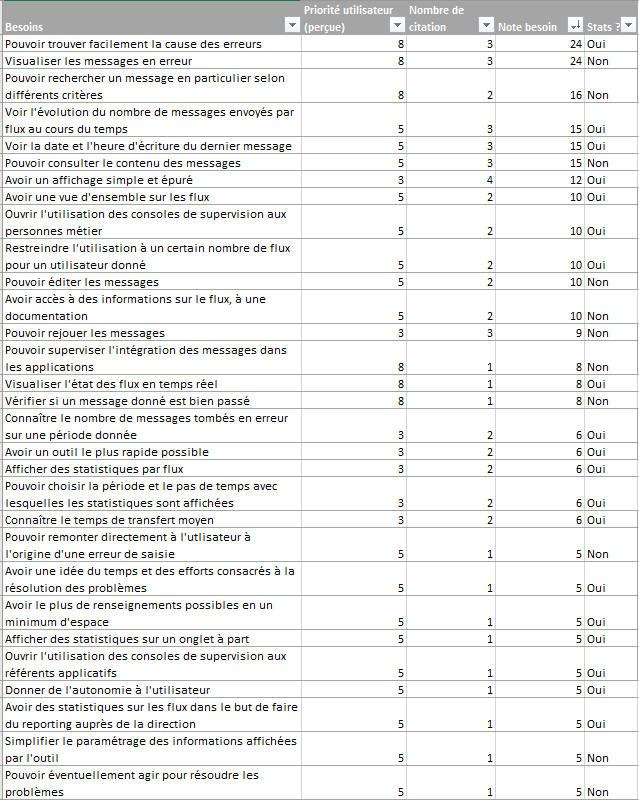
\includegraphics[width=17cm]{../img/annexes/besoins_1.png}
	\end{figure}
	\begin{figure}[H]
		\centering
		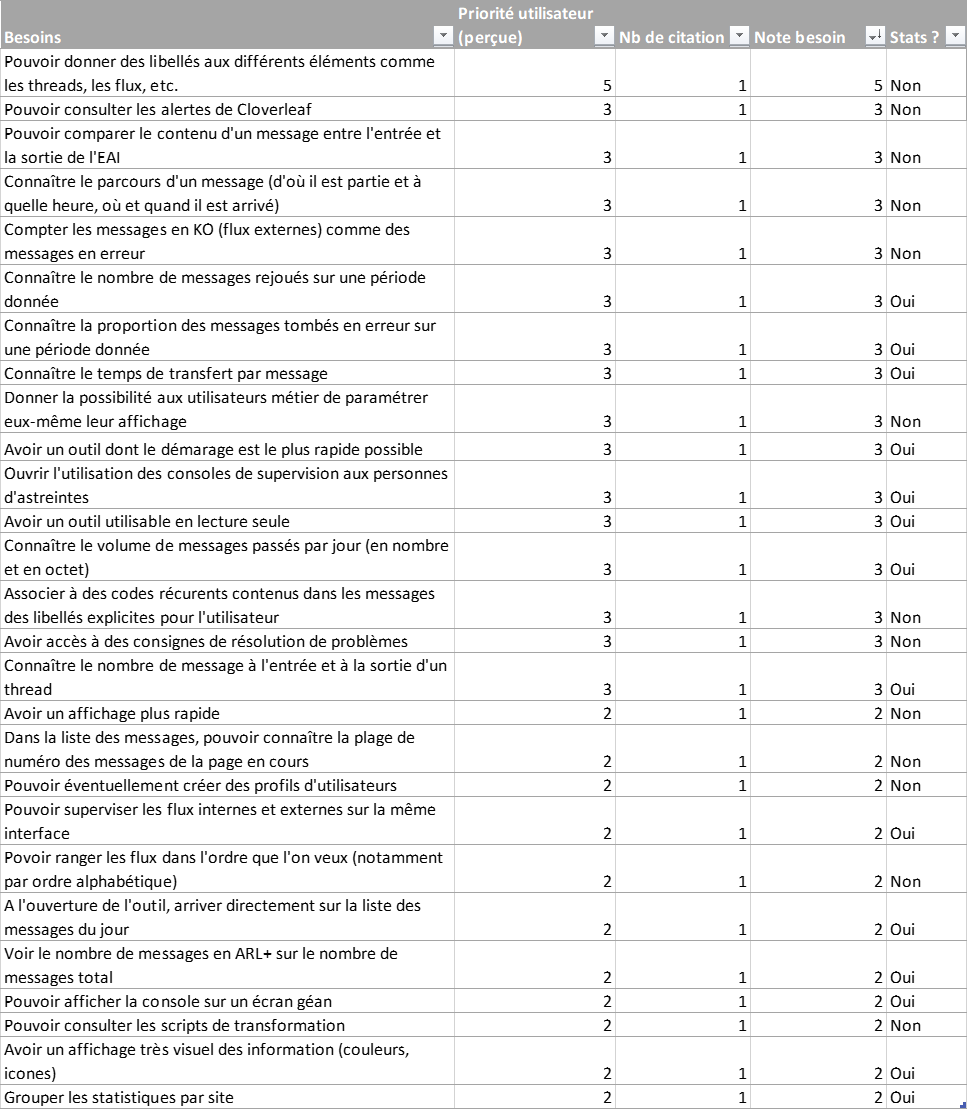
\includegraphics[width=17cm]{../img/annexes/besoins_2.png}
	\end{figure}
		\tocless\chapter{Liste des fonctionnalités}
	\begin{figure}[H]
		\centering
		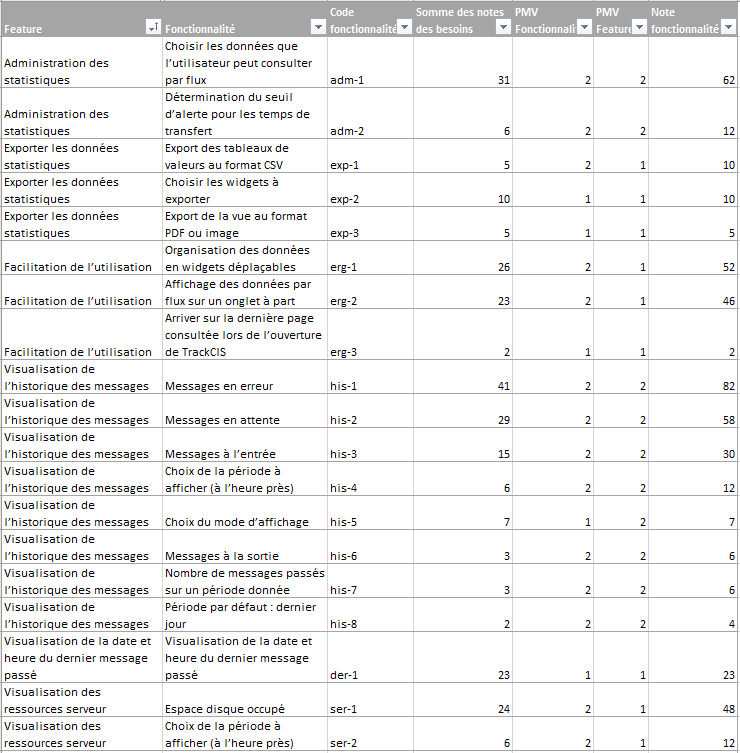
\includegraphics[width=17cm]{../img/annexes/fonctios_1.png}
	\end{figure}
	\begin{figure}[H]
		\centering
		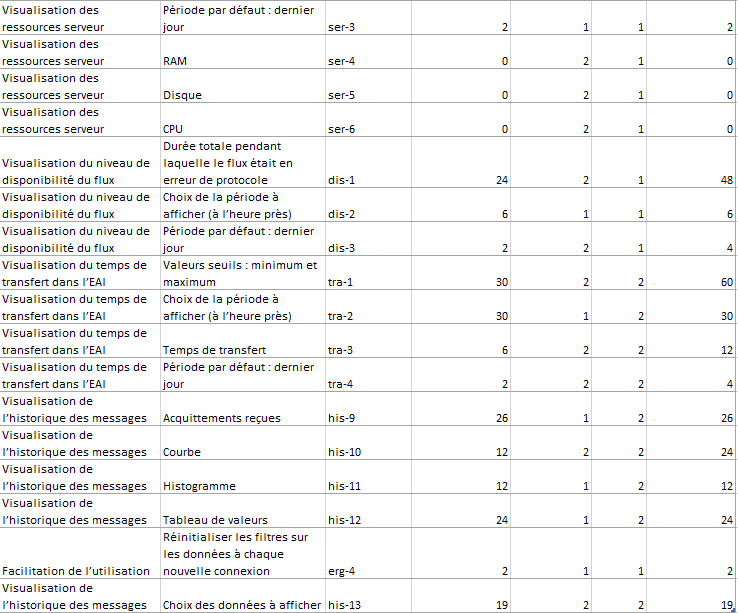
\includegraphics[width=17cm]{../img/annexes/fonctios_2.png}
	\end{figure}
		\tocless\chapter{Backlog}
	\begin{figure}[H]
		\centering
		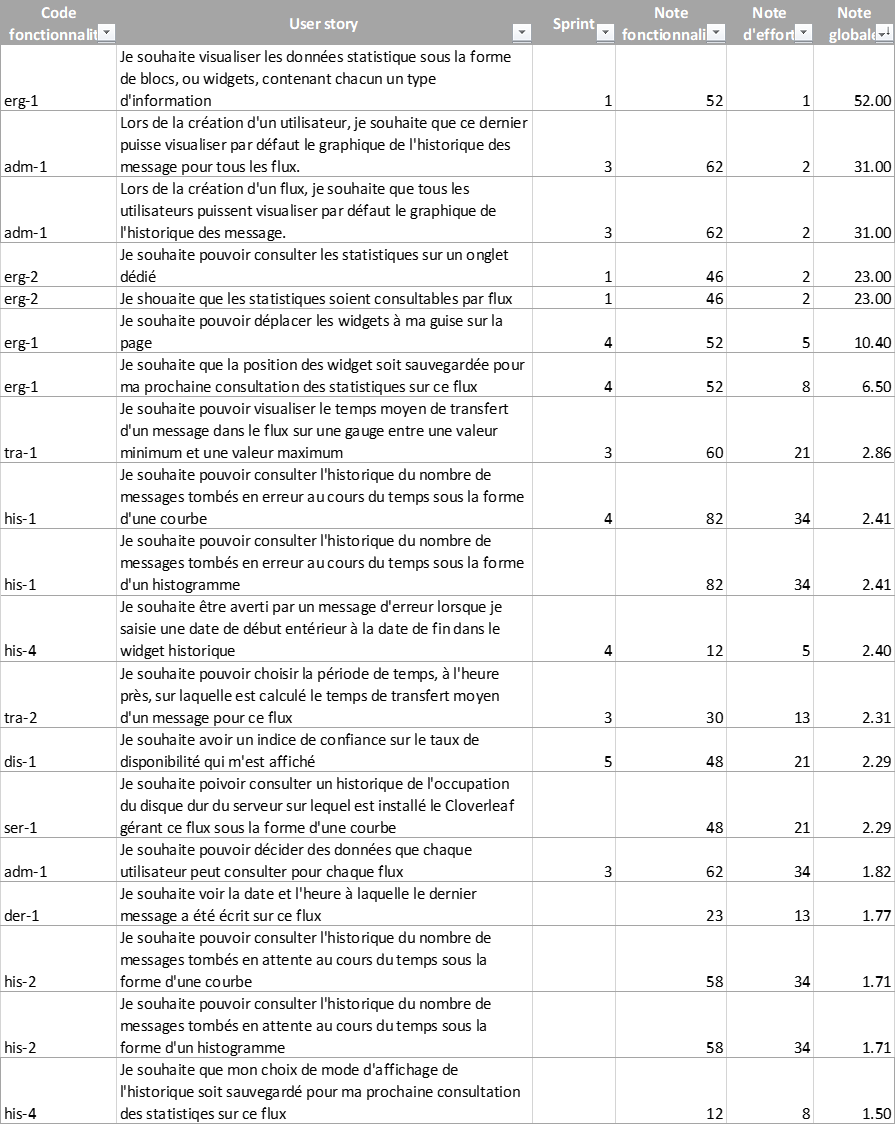
\includegraphics[width=17cm]{../img/annexes/backlog_1.png}
	\end{figure}
	\begin{figure}[H]
		\centering
		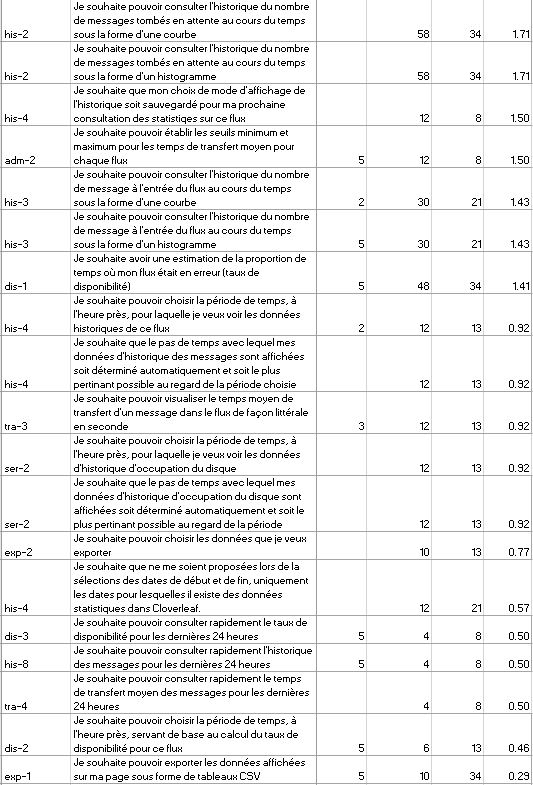
\includegraphics[width=17cm]{../img/annexes/backlog_2.png}
	\end{figure}
	\begin{figure}[H]
		\centering
		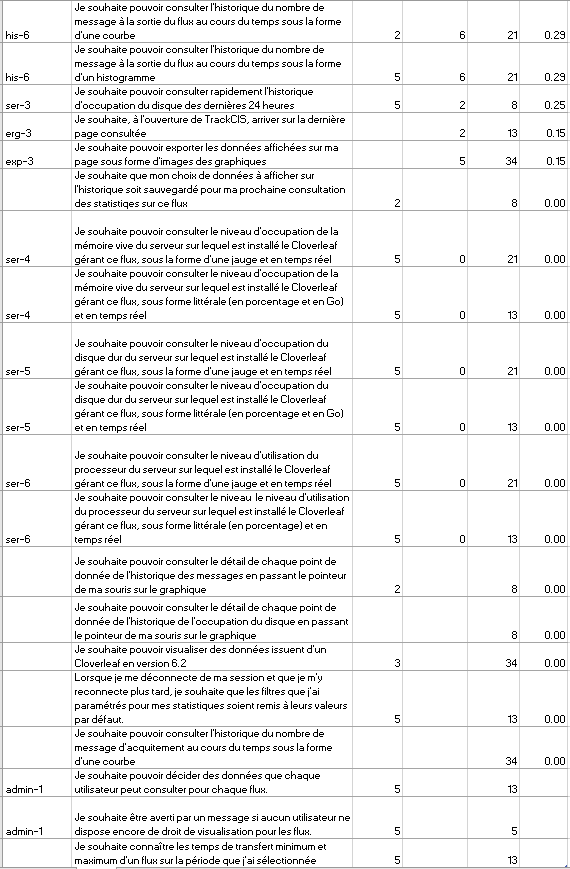
\includegraphics[width=17cm]{../img/annexes/backlog_3.png}
	\end{figure}
	\end{appendix}
	
	\newpage
	\thispagestyle{empty}
	\subsection{Résumé}
	\paragraph{}
	

\subsection{Abstract}
	\paragraph{}

\end{document}